%%%%%%%%%%%%%%%%%%%%%%%%%%%%%%%%%%%%%%%%%%%%%%%%%%%%%%%%%%%%%%%%%%%%%%%%%%%%%%%
%                                                                             %
% Copyright (C) 2015 Edward d'Auvergne                                        %
%                                                                             %
% This file is part of the program relax (http://www.nmr-relax.com).          %
%                                                                             %
% This program is free software: you can redistribute it and/or modify        %
% it under the terms of the GNU General Public License as published by        %
% the Free Software Foundation, either version 3 of the License, or           %
% (at your option) any later version.                                         %
%                                                                             %
% This program is distributed in the hope that it will be useful,             %
% but WITHOUT ANY WARRANTY; without even the implied warranty of              %
% MERCHANTABILITY or FITNESS FOR A PARTICULAR PURPOSE.  See the               %
% GNU General Public License for more details.                                %
%                                                                             %
% You should have received a copy of the GNU General Public License           %
% along with this program.  If not, see <http://www.gnu.org/licenses/>.       %
%                                                                             %
%%%%%%%%%%%%%%%%%%%%%%%%%%%%%%%%%%%%%%%%%%%%%%%%%%%%%%%%%%%%%%%%%%%%%%%%%%%%%%%


% Frame order models.
%%%%%%%%%%%%%%%%%%%%%

\chapter{The frame order models}
\label{ch: The frame order models}




% Intro.
%~~~~~~~

\section{The current frame order models}

In this advanced topic chapter, the equations for the various frame order models will be derived and validated using simulations.  The models include:
\begin{enumerate}
    \item Rigid
    \item Rotor
    \item Free rotor
    \item Isotropic cone
    \item Isotropic cone, torsionless
    \item Isotropic cone, free rotor
    \item Pseudo-ellipse
    \item Pseudo-ellipse, torsionless
    \item Pseudo-ellipse, free rotor
    \item Double rotor
\end{enumerate}

For a basic introduction to the frame order concept and the modelling of the tilt and torsion components, see Section~\ref{sect: Frame order modelling}.



% Simulation.
\section{Simulation of the frame order models}
\label{sect: frame order simulation}
\index{Frame order!simulation|textbf}

To validate the derived frame order matrix equations for the models, the real frame order matrix values for a given parameter set can be simulated.
The following script was used for simulating the isotropic cone and pseudo-ellipse frame order matrices.
As the other models are parametric restrictions of these two models, the simpler models were not simulated.
The script allows for both an `in\_frame' and `out\_of\_frame' or `axis2\_1\_3' mode to observe the components both within the motional eigenframe and in a rotated frame.
The value of \pycode{VAR} can be set to \pystring{ISO} for selecting the isotropic cone $\conetheta$ parameter to vary, or \pystring{X}, \pystring{Y}, or \pystring{Z} to vary the pseudo-ellipse $\conethetax$, $\conethetay$, and $\conesmax$ parameters respectively.

\lstinputlisting{frame_order/inf_frame_order.py}



% The rigid model.
\section{Rigid frame order model}
\index{Frame order!model!rigid|textbf}

% Rigid model parameterisation.
\subsection{Rigid model parameterisation}

This model consists solely of the six parameters of translation and rotation of the `moving' domain to its average position.
The parameter set is therefore
\begin{equation}
    \Modelset = \Posset = \Possetfull,
\end{equation}

where $\aveposi$ are the average domain position translations and rotations.


% Rigid model equations.
\subsection{Rigid model equations}

\subsubsection{Rigid model rotation matrices}

For the rigid model, there is no motion so the rotation matrix is simply the identity matrix
\begin{equation}
    R =
        \begin{pmatrix}
            1 & . & . \\
            . & 1 & . \\
            . & . & 1 \\
        \end{pmatrix}.
\end{equation}


\subsubsection{Rigid frame order matrix}
\index{Frame order!matrix}

The frame order matrix is
\begin{equation}
    \FOn = R^{\otimes n} ,
\end{equation}

where surface normalisation factor is 1.


\paragraph{Rigid \nth{1} degree frame order}

The \nth{1} degree frame order matrix with tensor rank-2 is the identity matrix
\begin{subequations} \label{eq: rigid 1st degree frame order matrix}
\begin{align}
    \FOone &= R^{\otimes 1} , \\
           &= \begin{pmatrix}
                  1 & . & . \\
                  . & 1 & . \\
                  . & . & 1 \\
              \end{pmatrix}.
\end{align}
\end{subequations}


\paragraph{Rigid \nth{2} degree frame order}

The \nth{2} degree frame order matrix with tensor rank-4 is the identity matrix
\begin{subequations} \label{eq: rigid 2nd degree frame order matrix}
\begin{align}
    \FOtwo &= R^{\otimes 2} , \\
           &= \begin{pmatrix}
                  1 & . & . & . & . & . & . & . & . \\
                  . & 1 & . & . & . & . & . & . & . \\
                  . & . & 1 & . & . & . & . & . & . \\
                  . & . & . & 1 & . & . & . & . & . \\
                  . & . & . & . & 1 & . & . & . & . \\
                  . & . & . & . & . & 1 & . & . & . \\
                  . & . & . & . & . & . & 1 & . & . \\
                  . & . & . & . & . & . & . & 1 & . \\
                  . & . & . & . & . & . & . & . & 1 \\
              \end{pmatrix}.
\end{align}
\end{subequations}



% The rotor model.
\section{Rotor frame order model}
\index{Frame order!model!rotor|textbf}

The rotor model is defined by its rotation axis and a pivot point to position the center of the rotation.


% Rotor model parameterisation.
\subsection{Rotor parameterisation}

The natural way to parameterise the rotation axis of rotor frame order model is to use a 3D point, the pivot point, and a unit vector using the spherical angle basis set.
This would result in the parameter set
\begin{subequations}
\begin{align}
    \Modelset &= \Eigensetax + \Pivotsetone, \\
              &= \Eigensetaxfull + \Pivotsetonefull.
\end{align}
\end{subequations}

However this is an overparameterisation as the point $\Pivotsetonefull$ can lie anywhere on the line defined by itself and the unit vector.
Due to computational truncation artifacts, this results in the pivot point shooting out to infinity along the line during optimisation.

The minimal set of independent parameters for the rotor model is four.
There are many parameterisation of lines in 3D using this minimal set of four parameters, however many of these suffer from singularity problems which can be fatal for optimisation.
By using geometry of the model together with information about the molecular system, a parameterisation can be constructed which avoid singularities:
\begin{itemize}
    \item A point of reference is the PDB frame close to the molecule is chosen, in this case the centre of mass (CoM) of the total system.
    \item The point on the line defining the rotation axis closest to the reference point defines an orthogonal system of the rotation axis to the vector of the CoM to closest point.  This point can be optimised with the parameters $\Pivotsetone = \Pivotsetonefull$ with no singularity problems and minimising truncation artifacts in the numerical PCS calculation.
    \item As the rotation axis is perpendicular to the CoM-$\Pivotsetone$ vector, it can be defined using a single angle of rotation ($\frameaxa$).  The reference starting point for the angle is arbitrarily set to the xy-plane.  The rotation of a unit vector about the CoM-$\Pivotsetone$ centred at $\Pivotsetone$ is smooth, hence singularities are also avoided.
\end{itemize}

The full parameter set for the rotor model implementation is therefore
\begin{subequations}
\begin{align}
    \Modelset &= \Posset + \Eigenseta + \Pivotsetone + \Orderset, \\
              &= \Possetfull + \Eigensetafull + \Pivotsetonefull + \left\{ \conesmax \right\},
\end{align}
\end{subequations}

where $\aveposi$ are the average domain position translations and rotations, $\frameaxa$ is the single angle defining the rotation axis, $\pivoti$ are the coordinates of the pivot point, and $\conesmax$ is the torsion half-angle of the rotor motion.

The rotation axis vector in the system is calculated as
\begin{equation}
    \raxhat = \left| R_\alpha \cdot (\rCoMpivhat \times \hat{z}) \right| .
\end{equation}

The angle $\frameaxa$ is obtained from $\raxhat$ as
\begin{subequations}
\begin{align}
    \frameaxa &= \frac{\pi}{2} - \arccos(\raxhat \cdot \hat{z}), \\
              &= \arcsin(\raxhat \cdot \hat{z}),
\end{align}
\end{subequations}


% Rotor model equations.
\subsection{Rotor equations}

The only motion is in the torsion angle about the rotation axis.

\begin{figure}
\centering
  \begin{tabular}{@{}cc@{}}
    \includegraphics[width=.5\textwidth]{images/frame_order_matrix/Sij_rotor_in_frame_theta_z_ens1000000.eps} &
    \includegraphics[width=.5\textwidth]{images/frame_order_matrix/Sij_rotor_in_frame_theta_z_calc.eps} \\
    \\[-5pt]
    \includegraphics[width=.5\textwidth]{images/frame_order_matrix/Sijkl_rotor_in_frame_theta_z_ens1000000.eps} &
    \includegraphics[width=.5\textwidth]{images/frame_order_matrix/Sijkl_rotor_in_frame_theta_z_calc.eps} \\
  \end{tabular}
  \caption[Rotor simulated and calculated in-frame Daeg$^{(1)}$ and Daeg$^{(2)}$ elements.]{
    The rotor model simulated and calculated in-frame $\FOone$ and $\FOtwo$ frame order matrix elements.
    The top row corresponds to $\FOone$ and the bottom to $\FOtwo$.
    In these plots, $\theta_{\textrm{Z}}$ corresponds to the torsion half-angle $\conesmax$.
    Frame order matrix values have been calculated every 10 degrees.
  }
  \label{fig: simulated and calculated in-frame 1st and 2nd degree rotor frame order}
\end{figure}

\begin{figure}
\centering
  \begin{tabular}{@{}cc@{}}
    \includegraphics[width=.5\textwidth]{images/frame_order_matrix/Sij_rotor_out_of_frame_theta_z_ens1000000.eps} &
    \includegraphics[width=.5\textwidth]{images/frame_order_matrix/Sij_rotor_out_of_frame_theta_z_calc.eps} \\
    \\[-5pt]
    \includegraphics[width=.5\textwidth]{images/frame_order_matrix/Sijkl_rotor_out_of_frame_theta_z_ens1000000.eps} &
    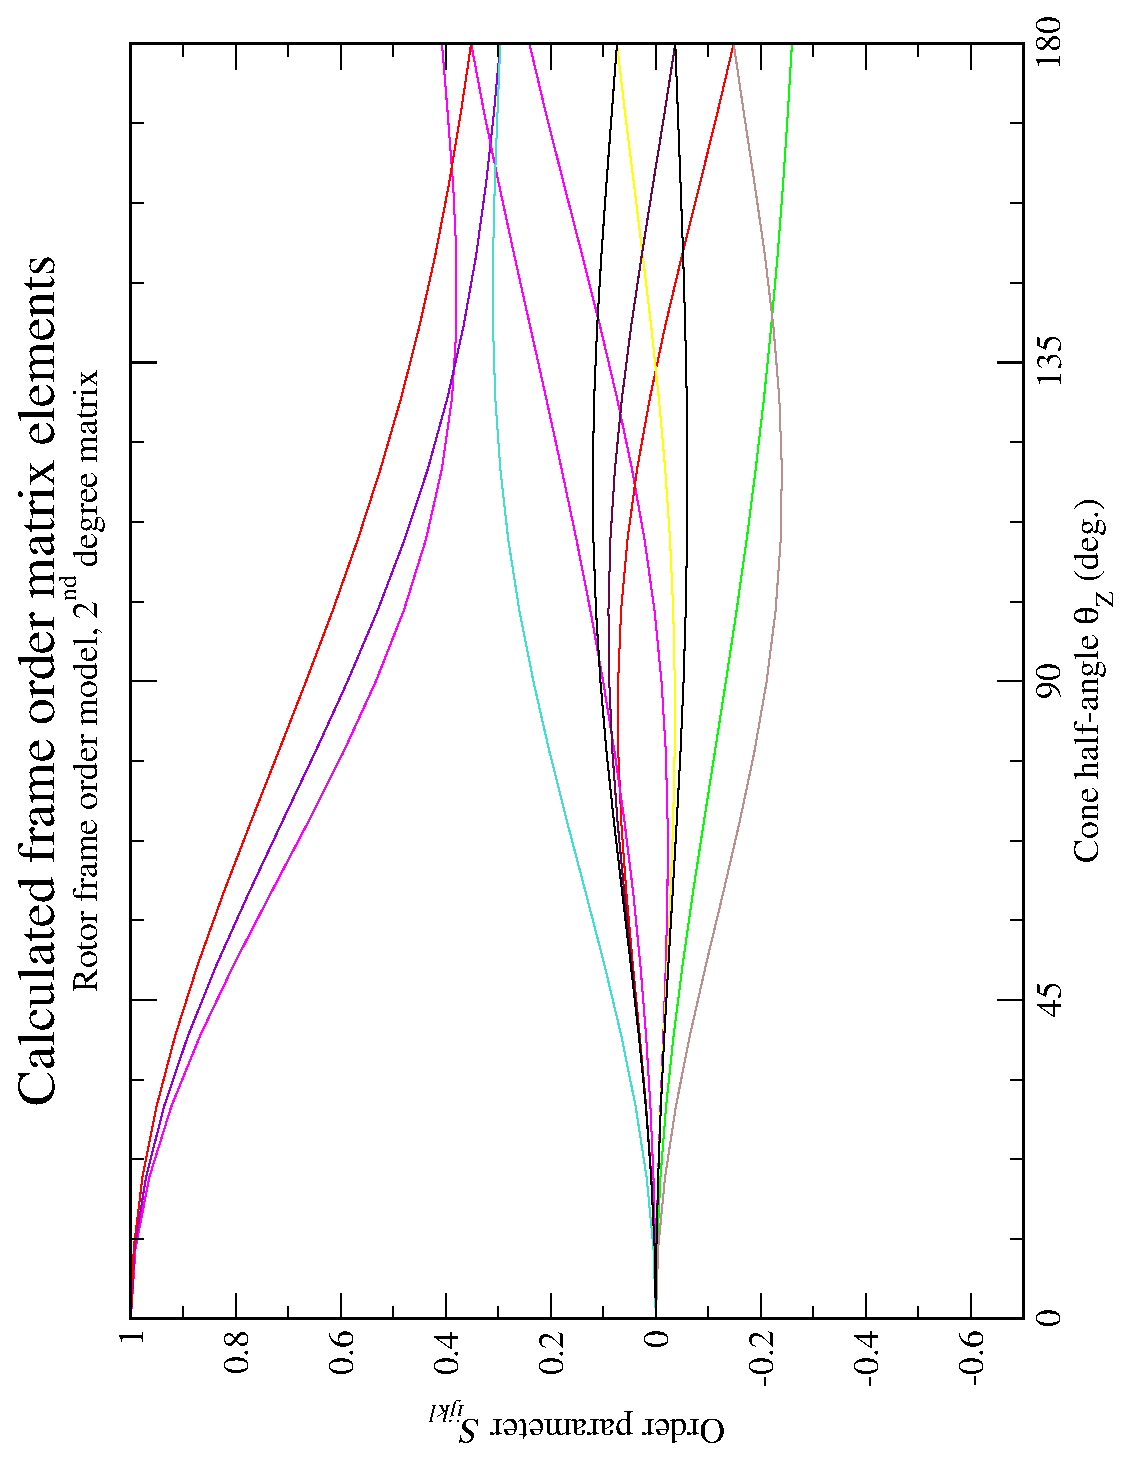
\includegraphics[width=.5\textwidth]{images/frame_order_matrix/Sijkl_rotor_out_of_frame_theta_z_calc.eps} \\
  \end{tabular}
  \caption[Rotor simulated and calculated out-of-frame Daeg$^{(1)}$ and Daeg$^{(2)}$ elements.]{
    The rotor model simulated and calculated out-of-frame $\FOone$ and $\FOtwo$ frame order matrix elements.
    The top row corresponds to $\FOone$ and the bottom to $\FOtwo$.
    In these plots, $\theta_{\textrm{Z}}$ corresponds to the torsion half-angle $\conesmax$.
    Frame order matrix values have been calculated every 10 degrees.
  }
  \label{fig: simulated and calculated out-of-frame 1st and 2nd degree rotor frame order}
\end{figure}


\subsubsection{Rotor rotation matrices}

Assuming the rotation axis is the z-axis, the rotation matrix is defined as
\begin{equation}\label{eq: R matrix torsion}
    R(\sigma) =
        \begin{pmatrix}
            \cos\sigma & -\sin\sigma & 0 \\
            \sin\sigma & \cos\sigma  & 0 \\
            0          & 0           & 1 \\
        \end{pmatrix}.
\end{equation}

\subsubsection{Rotor frame order matrix}
\index{Frame order!matrix}

The frame order matrix is
\begin{subequations}
\begin{align}
    \FOn &= \left. \int_S R^{\otimes n} \diff S \right / \int_S \diff S, \\
         &= \left. \int_{-\conesmax}^{\conesmax} R^{\otimes n} \diff \sigma  \right / \int_S \diff S.
\end{align}
\end{subequations}

The surface normalisation factor is
\begin{subequations}
\begin{align}
    \int_S \diff S &= \int_{-\conesmax}^{\conesmax} \diff \sigma , \\
                   &= 2\conesmax .
\end{align}
\end{subequations}


\paragraph{Rotor \nth{1} degree frame order}

The \nth{1} degree frame order matrix with tensor rank-2 is
\begin{subequations} \label{eq: rotor 1st degree frame order matrix}
\begin{align}
    \FOone &= \left. \int_S R^{\otimes 1} \diff S \right / \int_S \diff S, \\
           &= \left. \int_S R \diff S \right / 2\conesmax, \\
           &= \begin{pmatrix}
                  \sinc\conesmax & .              & . \\
                  .              & \sinc\conesmax & . \\
                  .              & .              & 1 \\
              \end{pmatrix} .
\end{align}
\end{subequations}


\paragraph{Rotor \nth{2} degree frame order}

The \nth{2} degree frame order matrix with tensor rank-4 is
\begin{subequations}
\begin{align}
    \FOtwo &= \left. \int_S R^{\otimes 2} \diff S \right / \int_S \diff S, \\
           &= \left. \int_S R \otimes R \diff S \right / 2\conesmax, \\
           &= \half \begin{pmatrix}
    \sinctwosigma+1  & .               & .           & .               & -\sinctwosigma+1 & .           & .           & .           & . \\
    .                & \sinctwosigma+1 & .           & \sinctwosigma-1 & .                & .           & .           & .           & . \\
    .                & .               & 2\sincsigma & .               & .                & .           & .           & .           & . \\
    .                & \sinctwosigma-1 & .           & \sinctwosigma+1 & .                & .           & .           & .           & . \\
    -\sinctwosigma+1 & .               & .           & .               & \sinctwosigma+1  & .           & .           & .           & . \\
    .                & .               & .           & .               & .                & 2\sincsigma & .           & .           & . \\
    .                & .               & .           & .               & .                & .           & 2\sincsigma & .           & . \\
    .                & .               & .           & .               & .                & .           & .           & 2\sincsigma & . \\
    .                & .               & .           & .               & .                & .           & .           & .           & 1 \\
              \end{pmatrix} ,
\end{align}
\end{subequations}

where $\sincsigma = \sinc\conesmax$ and $\sinctwosigma = \sinc(2\conesmax)$.
The active matrix elements which are not zero due to symmetries, in Kronecker product double indices from 0 to 8, are
\begin{subequations} \label{eq: rotor 2nd degree frame order matrix}
\begin{align}
    &\FO_{00} = \half\sinc(2\conesmax) + \half , \\
    &\FO_{11} = \FO_{00} , \\
    &\FO_{22} = \sinc\conesmax , \\
    &\FO_{33} = \FO_{00} , \\
    &\FO_{44} = \FO_{00} , \\
    &\FO_{55} = \FO_{22} , \\
    &\FO_{66} = \FO_{22} , \\
    &\FO_{77} = \FO_{22} , \\
    &\FO_{88} = 1 , \\
    &\FO_{04} = -\half\sinc(2\conesmax) + \half , \\
    &\FO_{40} = \FO_{04} , \\
    &\FO_{08} = 0 , \\
    &\FO_{80} = 0 , \\
    &\FO_{48} = 0 , \\
    &\FO_{84} = 0 , \\
    &\FO_{13} = -\FO_{04} , \\
    &\FO_{31} = -\FO_{04} , \\
    &\FO_{26} = 0 , \\
    &\FO_{62} = 0 , \\
    &\FO_{57} = 0 , \\
    &\FO_{75} = 0 .
\end{align}
\end{subequations}


\subparagraph[Frame order matrix simulation and calculation]{Rotor frame order matrix simulation and calculation}

The frame order matrix element simulation script from Section~\ref{sect: frame order simulation}, page~\pageref{sect: frame order simulation} was used to compare the implementation of equations~\ref{eq: rotor 1st degree frame order matrix} and~\ref{eq: rotor 2nd degree frame order matrix} above.
Frame order matrix $\FOone$ and $\FOtwo$ values were both simulated and calculated, both within and out of the motional eigenframe.
The in-frame $\FOone$ and $\FOtwo$ values are shown in figure~\ref{fig: simulated and calculated in-frame 1st and 2nd degree rotor frame order}.
The out-of-frame $\FOone$ and $\FOtwo$ values are shown in figure~\ref{fig: simulated and calculated out-of-frame 1st and 2nd degree rotor frame order}.



% The free rotor model.
\section{Free rotor frame order model}
\index{Frame order!model!free rotor|textbf}

This is similar to the rotor model but with no torsional restriction ($\conesmax = \pi$).


% Free rotor model parameterisation.
\subsection{Free rotor parameterisation}

The full parameter set for the free-rotor model implementation is
\begin{subequations}
\begin{align}
    \Modelset &= \Posset + \Eigenseta + \Pivotsetone, \\
              &= \Possetfull + \Eigensetafull + \Pivotsetonefull,
\end{align}
\end{subequations}

where $\aveposi$ are the average domain position translations and rotations, $\frameaxa$ is the single angle defining the rotation axis, and $\pivoti$ are the coordinates of the pivot point.


% Free rotor model equations.
\subsection{Free rotor equations}

\begin{figure}
\centering
  \begin{tabular}{@{}cc@{}}
    \includegraphics[width=.5\textwidth]{images/frame_order_matrix/Sij_free_rotor_in_frame_theta_z_ens1000000.eps} &
    \includegraphics[width=.5\textwidth]{images/frame_order_matrix/Sij_free_rotor_in_frame_theta_z_calc.eps} \\
    \\[-5pt]
    \includegraphics[width=.5\textwidth]{images/frame_order_matrix/Sijkl_free_rotor_in_frame_theta_z_ens1000000.eps} &
    \includegraphics[width=.5\textwidth]{images/frame_order_matrix/Sijkl_free_rotor_in_frame_theta_z_calc.eps} \\
  \end{tabular}
  \caption[Free rotor simulated and calculated in-frame Daeg$^{(1)}$ and Daeg$^{(2)}$ elements.]{
    The free rotor model simulated and calculated in-frame $\FOone$ and $\FOtwo$ frame order matrix elements.
    The top row corresponds to $\FOone$ and the bottom to $\FOtwo$.
    In these plots, as no motional order parameters exist for the model, $\theta_{\textrm{Z}}$ corresponds to nothing.
    Frame order matrix values have been calculated every 10 degrees.
  }
  \label{fig: simulated and calculated in-frame 1st and 2nd degree free rotor frame order}
\end{figure}

\begin{figure}
\centering
  \begin{tabular}{@{}cc@{}}
    \includegraphics[width=.5\textwidth]{images/frame_order_matrix/Sij_free_rotor_out_of_frame_theta_z_ens1000000.eps} &
    \includegraphics[width=.5\textwidth]{images/frame_order_matrix/Sij_free_rotor_out_of_frame_theta_z_calc.eps} \\
    \\[-5pt]
    \includegraphics[width=.5\textwidth]{images/frame_order_matrix/Sijkl_free_rotor_out_of_frame_theta_z_ens1000000.eps} &
    \includegraphics[width=.5\textwidth]{images/frame_order_matrix/Sijkl_free_rotor_out_of_frame_theta_z_calc.eps} \\
  \end{tabular}
  \caption[Free rotor simulated and calculated out-of-frame Daeg$^{(1)}$ and Daeg$^{(2)}$ elements.]{
    The free rotor model simulated and calculated out-of-frame $\FOone$ and $\FOtwo$ frame order matrix elements.
    The top row corresponds to $\FOone$ and the bottom to $\FOtwo$.
    In these plots, as no motional order parameters exist for the model, $\theta_{\textrm{Z}}$ corresponds to nothing.
    Frame order matrix values have been calculated every 10 degrees.
  }
  \label{fig: simulated and calculated out-of-frame 1st and 2nd degree free rotor frame order}
\end{figure}

\subsubsection{Free rotor rotation matrices}

The rotation matrix is defined in equation~\ref{eq: R matrix torsion}.

\subsubsection{Free rotor frame order matrix}
\index{Frame order!matrix}

The frame order matrix is
\begin{subequations}
\begin{align}
    \FOn &= \left. \int_S R^{\otimes n} \diff S \right / \int_S \diff S , \\
         &= \left. \int_{-\pi}^{\pi} R^{\otimes n} \diff \sigma  \right / \int_S \diff S .
\end{align}
\end{subequations}

The surface normalisation factor is
\begin{subequations}
\begin{align}
    \int_S \diff S &= \int_{-\pi}^{\pi} \diff \sigma , \\
                   &= 2\pi .
\end{align}
\end{subequations}


\paragraph{Free rotor \nth{1} degree frame order}

The \nth{1} degree frame order matrix with tensor rank-2 is
\begin{subequations} \label{eq: free rotor 1st degree frame order matrix}
\begin{align}
    \FOone &= \left. \int_S R^{\otimes 1} \diff S \right / \int_S \diff S, \\
           &= \left. \int_S R \diff S \right / 2\pi, \\
           &= \begin{pmatrix}
                  . & . & . \\
                  . & . & . \\
                  . & . & 1 \\
              \end{pmatrix} .
\end{align}
\end{subequations}


\paragraph{Free rotor \nth{2} degree frame order}

The frame order matrix in Kronecker product notation is fixed as
\begin{equation} \label{eq: free rotor 2nd degree frame order matrix}
    \FOtwo =
        \begin{pmatrix}
            \half & .      & . & .      & \half & . & . & . & . \\
            .     & \half  & . & -\half & .     & . & . & . & . \\
            .     & .      & . & .      & .     & . & . & . & . \\
            .     & -\half & . & \half  & .     & . & . & . & . \\
            \half & .      & . & .      & \half & . & . & . & . \\
            .     & .      & . & .      & .     & . & . & . & . \\
            .     & .      & . & .      & .     & . & . & . & . \\
            .     & .      & . & .      & .     & . & . & . & . \\
            .     & .      & . & .      & .     & . & . & . & 1 \\
        \end{pmatrix} .
\end{equation}


\subparagraph[Frame order matrix simulation and calculation]{Free rotor frame order matrix simulation and calculation}

The frame order matrix element simulation script from Section~\ref{sect: frame order simulation}, page~\pageref{sect: frame order simulation} was used to compare the implementation of equations~\ref{eq: free rotor 1st degree frame order matrix} and~\ref{eq: free rotor 2nd degree frame order matrix} above.
Frame order matrix $\FOone$ and $\FOtwo$ values were both simulated and calculated, both within and out of the motional eigenframe.
The in-frame $\FOone$ and $\FOtwo$ values are shown in figure~\ref{fig: simulated and calculated in-frame 1st and 2nd degree free rotor frame order}.
The out-of-frame $\FOone$ and $\FOtwo$ values are shown in figure~\ref{fig: simulated and calculated out-of-frame 1st and 2nd degree free rotor frame order}.



% The isotropic cone model.
\section{Isotropic cone frame order model}
\index{Frame order!model!isotropic cone|textbf}





% Isotropic cone model parameterisation.
%---------------------------------------

\subsection{Isotropic cone parameterisation}

In this model, the tilt component of the tilt and torsion angle system is modelled simply as
\begin{equation}
    \theta \le \conethetamax .
\end{equation}

The torsion angle restriction of~\ref{eq: torsion angle restriction} on page~\pageref{eq: torsion angle restriction} is used for the modelling of the torsion component.
A uniform distribution of rigid body positions within these bounds is assumed.

The isotropic cone model of the ball and socket joint consists of a single pivot point, a single unit z-vector of the motional eigenframe defining the cone axis, and the maximum cone opening and torsion half-angles.
Including the average domain position, the parameter set is therefore
\begin{subequations}
\begin{align}
    \Modelset &= \Posset + \Eigensetax + \Pivotsetone + \Orderset, \\
              &= \Possetfull + \Eigensetaxfull + \Pivotsetonefull + \left\{ \conethetamax, \conesmax \right\} ,
\end{align}
\end{subequations}

where $\aveposi$ are the average domain position translations and rotations, $\framei$ are the spherical angles defining the cone axis, $\pivoti$ are the coordinates of the pivot point, and $\conethetamax$ and $\conesmax$ are the maximum cone opening and torsion half-angles respectively.




% Isotropic cone model equations.
\subsection{Isotropic cone equations}

\begin{figure}
\centering
  \begin{tabular}{@{}cc@{}}
    \includegraphics[width=.5\textwidth]{images/frame_order_matrix/Sij_iso_cone_in_frame_theta_x_ens1000000.eps} &
    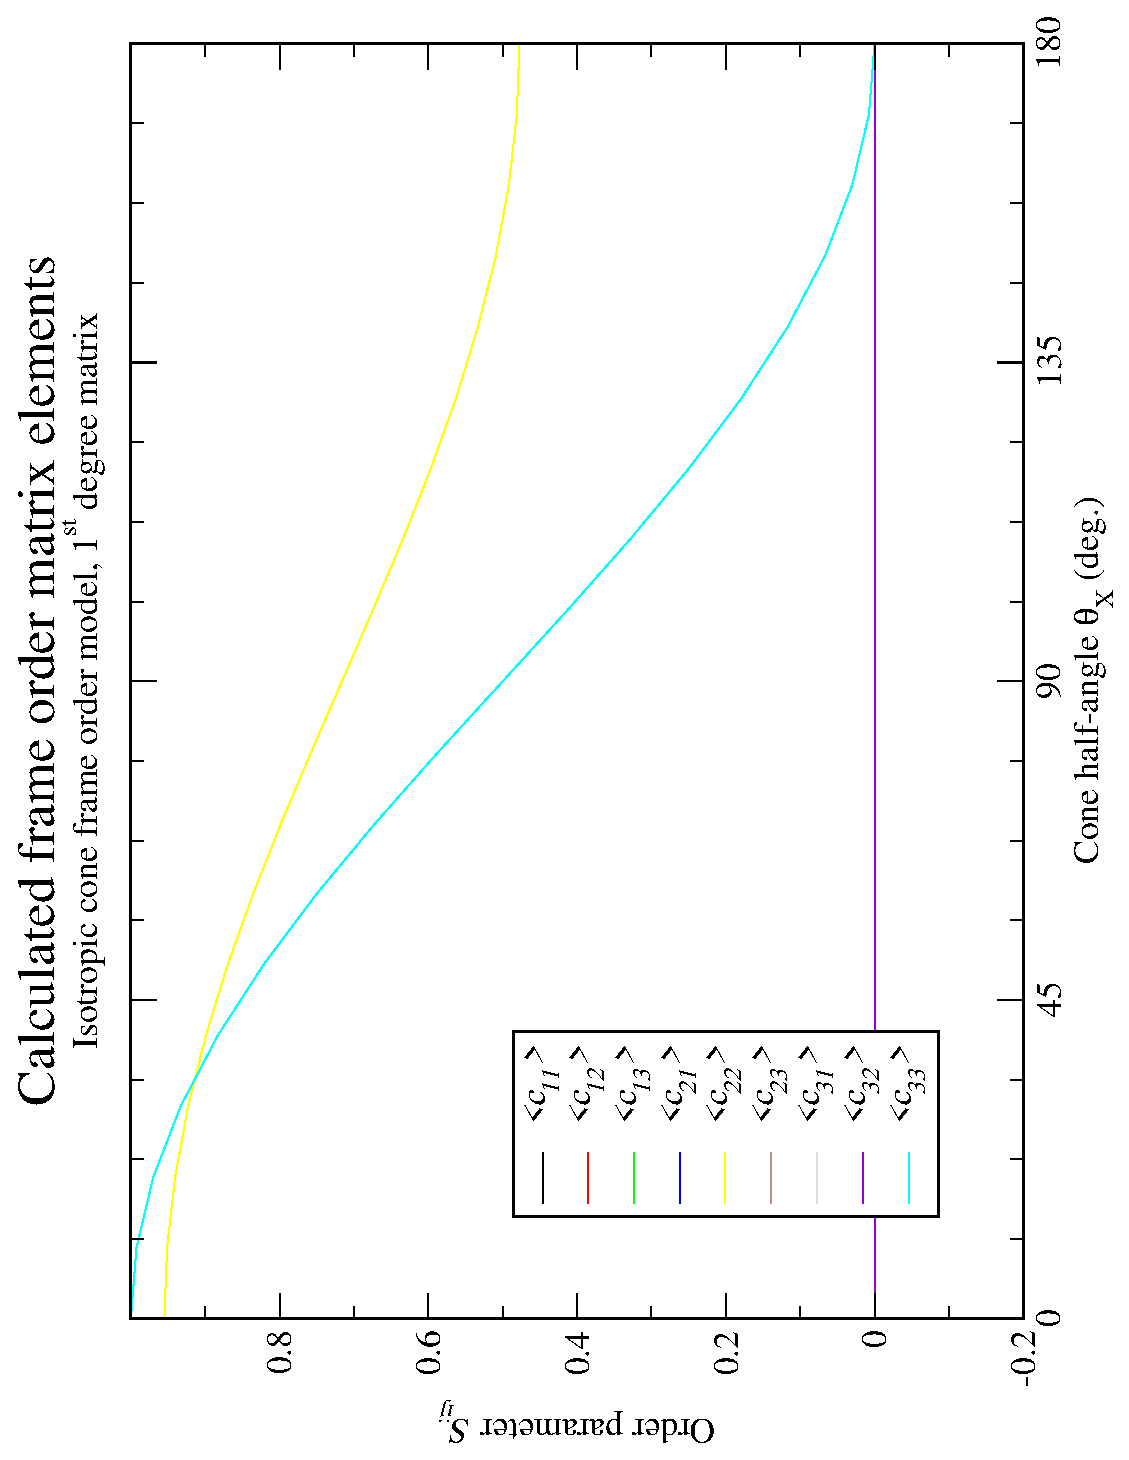
\includegraphics[width=.5\textwidth]{images/frame_order_matrix/Sij_iso_cone_in_frame_theta_x_calc.eps} \\
    \\[-5pt]
    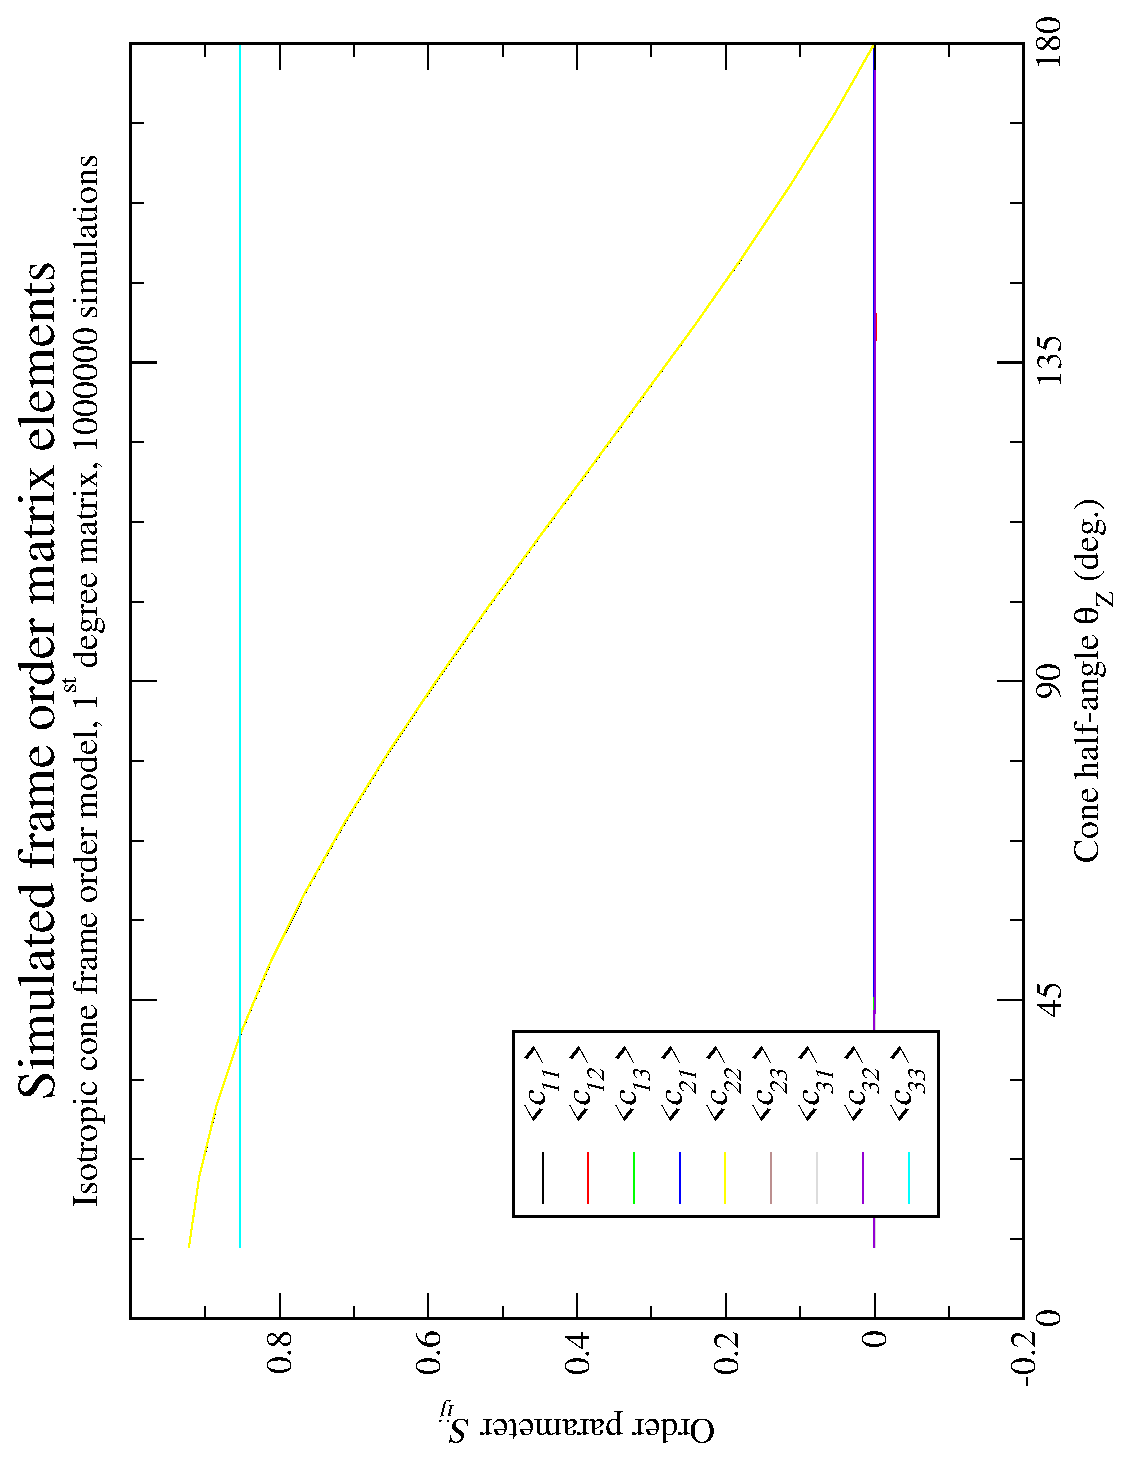
\includegraphics[width=.5\textwidth]{images/frame_order_matrix/Sij_iso_cone_in_frame_theta_z_ens1000000.eps} &
    \includegraphics[width=.5\textwidth]{images/frame_order_matrix/Sij_iso_cone_in_frame_theta_z_calc.eps} \\
  \end{tabular}
  \caption[Isotropic cone simulated and calculated in-frame Daeg$^{(1)}$ elements.]{
    The isotropic cone model simulated and calculated in-frame $\FOone$ frame order matrix elements.
    In these plots, $\theta_{\textrm{X}}$ corresponds to the cone opening half-angle $\conetheta$ and $\theta_{\textrm{Z}}$ to the torsion half-angle $\conesmax$.
    When the half-angle is not varied, the angle is fixed to either $\conetheta = \pi/4$ or $\conesmax = \pi/6$.
    Frame order matrix values have been calculated every 10 degrees.
  }
  \label{fig: simulated and calculated in-frame 1st degree iso cone frame order}
\end{figure}

\begin{figure}
\centering
  \begin{tabular}{@{}cc@{}}
    \includegraphics[width=.5\textwidth]{images/frame_order_matrix/Sijkl_iso_cone_in_frame_theta_x_ens1000000.eps} &
    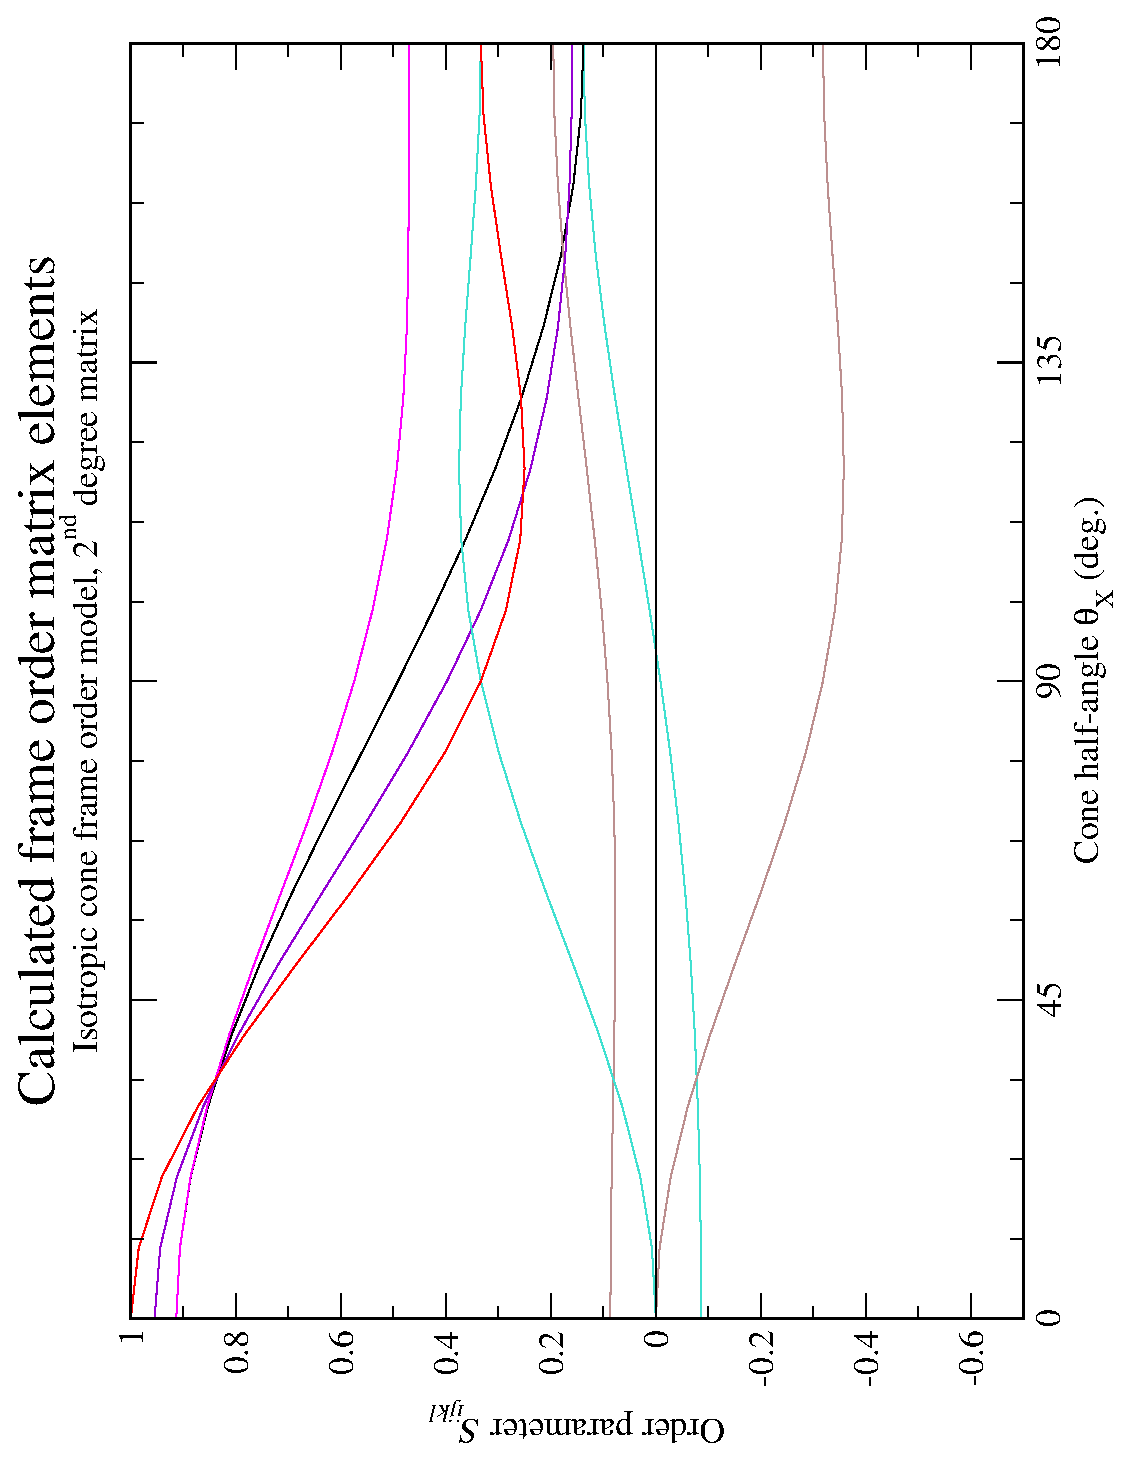
\includegraphics[width=.5\textwidth]{images/frame_order_matrix/Sijkl_iso_cone_in_frame_theta_x_calc.eps} \\
    \\[-5pt]
    \includegraphics[width=.5\textwidth]{images/frame_order_matrix/Sijkl_iso_cone_in_frame_theta_z_ens1000000.eps} &
    \includegraphics[width=.5\textwidth]{images/frame_order_matrix/Sijkl_iso_cone_in_frame_theta_z_calc.eps} \\
  \end{tabular}
  \caption[Isotropic cone simulated and calculated in-frame Daeg$^{(2)}$ elements.]{
    The isotropic cone model simulated and calculated in-frame $\FOtwo$ frame order matrix elements.
    In these plots, $\theta_{\textrm{X}}$ corresponds to the cone opening half-angle $\conetheta$ and $\theta_{\textrm{Z}}$ to the torsion half-angle $\conesmax$.
    When the half-angle is not varied, the angle is fixed to either $\conetheta = \pi/4$ or $\conesmax = \pi/6$.
    Frame order matrix values have been calculated every 10 degrees.
  }
  \label{fig: simulated and calculated in-frame 2nd degree iso cone frame order}
\end{figure}

\begin{figure}
\centering
  \begin{tabular}{@{}cc@{}}
    \includegraphics[width=.5\textwidth]{images/frame_order_matrix/Sij_iso_cone_out_of_frame_theta_x_ens1000000.eps} &
    \includegraphics[width=.5\textwidth]{images/frame_order_matrix/Sij_iso_cone_out_of_frame_theta_x_calc.eps} \\
    \\[-5pt]
    \includegraphics[width=.5\textwidth]{images/frame_order_matrix/Sij_iso_cone_out_of_frame_theta_z_ens1000000.eps} &
    \includegraphics[width=.5\textwidth]{images/frame_order_matrix/Sij_iso_cone_out_of_frame_theta_z_calc.eps} \\
  \end{tabular}
  \caption[Isotropic cone simulated and calculated out-of-frame Daeg$^{(1)}$ elements.]{
    The isotropic cone model simulated and calculated out-of-frame $\FOone$ frame order matrix elements.
    In these plots, $\theta_{\textrm{X}}$ corresponds to the cone opening half-angle $\conetheta$ and $\theta_{\textrm{Z}}$ to the torsion half-angle $\conesmax$.
    When the half-angle is not varied, the angle is fixed to either $\conetheta = \pi/4$ or $\conesmax = \pi/6$.
    Frame order matrix values have been calculated every 10 degrees.
  }
  \label{fig: simulated and calculated out-of-frame 1st degree iso cone frame order}
\end{figure}

\begin{figure}
\centering
  \begin{tabular}{@{}cc@{}}
    \includegraphics[width=.5\textwidth]{images/frame_order_matrix/Sijkl_iso_cone_out_of_frame_theta_x_ens1000000.eps} &
    \includegraphics[width=.5\textwidth]{images/frame_order_matrix/Sijkl_iso_cone_out_of_frame_theta_x_calc.eps} \\
    \\[-5pt]
    \includegraphics[width=.5\textwidth]{images/frame_order_matrix/Sijkl_iso_cone_out_of_frame_theta_z_ens1000000.eps} &
    \includegraphics[width=.5\textwidth]{images/frame_order_matrix/Sijkl_iso_cone_out_of_frame_theta_z_calc.eps} \\
  \end{tabular}
  \caption[Isotropic cone simulated and calculated out-of-frame Daeg$^{(2)}$ elements.]{
    The isotropic cone model simulated and calculated out-of-frame $\FOtwo$ frame order matrix elements.
    In these plots, $\theta_{\textrm{X}}$ corresponds to the cone opening half-angle $\conetheta$ and $\theta_{\textrm{Z}}$ to the torsion half-angle $\conesmax$.
    When the half-angle is not varied, the angle is fixed to either $\conetheta = \pi/4$ or $\conesmax = \pi/6$.
    Frame order matrix values have been calculated every 10 degrees.
  }
  \label{fig: simulated and calculated out-of-frame 2nd degree iso cone frame order}
\end{figure}


\subsubsection{Isotropic cone rotation matrices}

The rotation matrix is the full torsion-tilt rotation matrix of equation~\ref{eq: R torsion-tilt} on page~\pageref{eq: R torsion-tilt}.


\subsubsection{Isotropic cone frame order matrix}
\index{Frame order!matrix}


The frame order matrix is
\begin{subequations}
\begin{align}
    \FOn &= \left. \int_S R^{\otimes n} \diff S \right / \int_S \diff S , \\
         &= \left. \int_{-\conesmax}^{\conesmax} \int_{-\pi}^{\pi} \int_{0}^{\conethetamax} R^{\otimes n} \sin\theta \diff\theta \diff\phi \diff\sigma  \right / \int_S \diff S .
\end{align}
\end{subequations}

The surface normalisation factor is
\begin{subequations}
\begin{align}
    \int_S \diff S &= \int_{-\conesmax}^{\conesmax} \int_{-\pi}^{\pi} \int_{0}^{\conethetamax} \sin\theta \diff\theta \diff\phi \diff\sigma , \\
                   &= \int_{-\conesmax}^{\conesmax} \int_{-\pi}^{\pi} \left( 1 - \cos\conethetamax \right) \diff\phi \diff\sigma , \\
                   &= \int_{-\conesmax}^{\conesmax} 2\pi \left( 1 - \cos\conethetamax \right) \diff\sigma , \\
                   &= 4\pi \conesmax \left( 1 - \cos\conethetamax \right) .
\end{align}
\end{subequations}


\paragraph{Isotropic cone \nth{1} degree frame order}

The \nth{1} degree frame order matrix with tensor rank-2 is
\begin{subequations} \label{eq: iso cone 1st degree frame order matrix}
\begin{align}
    \FOone &= \left. \int_S R^{\otimes 1} \diff S \right / \int_S \diff S , \\
           &= \left. \int_S R \diff S \right / 4\pi \conesmax \left( 1 - \cos\conethetamax \right) , \\
           &= \quart \begin{pmatrix}
                  \sinc\conesmax \left( \cos\conethetamax + 3 \right) & .                                                   & . \\
                  .                                                   & \sinc\conesmax \left( \cos\conethetamax + 3 \right) & . \\
                  .                                                   & .                                                   & 2\cos\conethetamax + 2 \\
              \end{pmatrix} .
\end{align}
\end{subequations}


\paragraph{Isotropic cone \nth{2} degree frame order}

The \nth{2} degree frame order matrix with tensor rank-4 consists of the following elements, using Kronecker product double indices from 0 to 8
\begin{subequations} \label{eq: iso cone 2nd degree frame order matrix}
\begin{align}
    &\FO_{00} = \tfrac{1}{24} \sinc(2\conesmax) \left( \cos^2\conethetamax + 4\cos\conethetamax + 7 \right)  +  \tfrac{1}{12} \left( \cos^2\conethetamax + \cos\conethetamax + 4 \right) , \\
    &\FO_{11} = \tfrac{1}{24} \sinc(2\conesmax) \left( \cos^2\conethetamax + 4\cos\conethetamax + 7 \right)  + \quart \left( \cos\conethetamax + 1 \right), \\
    &\FO_{22} = \tfrac{1}{12} \sinc(2\conesmax) \left( 2\cos^2\conethetamax + 5\cos\conethetamax + 5 \right) , \\
    &\FO_{33} = \FO_{11} , \\
    &\FO_{44} = \FO_{00} , \\
    &\FO_{55} = \FO_{22} , \\
    &\FO_{66} = \FO_{22} , \\
    &\FO_{77} = \FO_{22} , \\
    &\FO_{88} = \tfrac{1}{3} \left( \cos^2\conethetamax + \cos\conethetamax + 1 \right) , \\
    &\FO_{04} = -\tfrac{1}{24} \sinc(2\conesmax) \left( \cos^2\conethetamax + 4\cos\conethetamax + 7 \right)  +  \tfrac{1}{12} \left( \cos^2\conethetamax + \cos\conethetamax + 4 \right) , \\
    &\FO_{40} = \FO_{04} , \\
    &\FO_{08} = -\tfrac{1}{6} \left( \cos^2\conethetamax + \cos\conethetamax - 2 \right) , \\
    &\FO_{80} = \FO_{08} , \\
    &\FO_{48} = \FO_{08} , \\
    &\FO_{84} = \FO_{08} , \\
    &\FO_{13} = \tfrac{1}{24} \sinc(2\conesmax) \left( \cos^2\conethetamax + 4\cos\conethetamax + 7 \right)  -  \quart \left( \cos\conethetamax + 1 \right) , \\
    &\FO_{31} = \FO_{13} , \\
    &\FO_{26} = \tfrac{1}{6} \sinc(2\conesmax) \left( \cos^2\conethetamax + \cos\conethetamax - 2 \right) , \\
    &\FO_{62} = \FO_{26} , \\
    &\FO_{57} = \FO_{26} , \\
    &\FO_{75} = \FO_{26} .
\end{align}
\end{subequations}


\subparagraph[Frame order matrix simulation and calculation]{Isotropic cone frame order matrix simulation and calculation}

The frame order matrix element simulation script from Section~\ref{sect: frame order simulation}, page~\pageref{sect: frame order simulation} was used to compare the implementation of equations~\ref{eq: iso cone 1st degree frame order matrix} and~\ref{eq: iso cone 2nd degree frame order matrix} above.
Frame order matrix $\FOone$ and $\FOtwo$ values were both simulated and calculated, both within and out of the motional eigenframe.
The in-frame $\FOone$ values are shown in figure~\ref{fig: simulated and calculated in-frame 1st degree iso cone frame order} and $\FOtwo$ in figure~\ref{fig: simulated and calculated in-frame 2nd degree iso cone frame order}.
The out-of-frame $\FOone$ values are shown in figure~\ref{fig: simulated and calculated out-of-frame 1st degree iso cone frame order} and $\FOtwo$ in figure~\ref{fig: simulated and calculated out-of-frame 2nd degree iso cone frame order}.



% The torsionless isotropic cone model.
\section{Torsionless isotropic cone frame order model}
\index{Frame order!model!isotropic cone, torsionless|textbf}


% Torsionless isotropic cone model parameterisation.
\subsection{Torsionless isotropic cone parameterisation}

As this is simply the isotropic cone model with the torsion angle set to zero, $\conesmax = 0$, the models parameters are
\begin{subequations}
\begin{align}
    \Modelset &= \Posset + \Eigensetax + \Pivotsetone + \Orderset, \\
              &= \Possetfull + \Eigensetaxfull + \Pivotsetonefull + \left\{ \conethetamax \right\} ,
\end{align}
\end{subequations}

where $\aveposi$ are the average domain position translations and rotations, $\framei$ are the spherical angles defining the cone axis, $\pivoti$ are the coordinates of the pivot point, and $\conethetamax$ is the maximum cone opening half-angle.


% Torsionless isotropic cone model equations.
\subsection{Torsionless isotropic cone equations}

\begin{figure}
\centering
  \begin{tabular}{@{}cc@{}}
    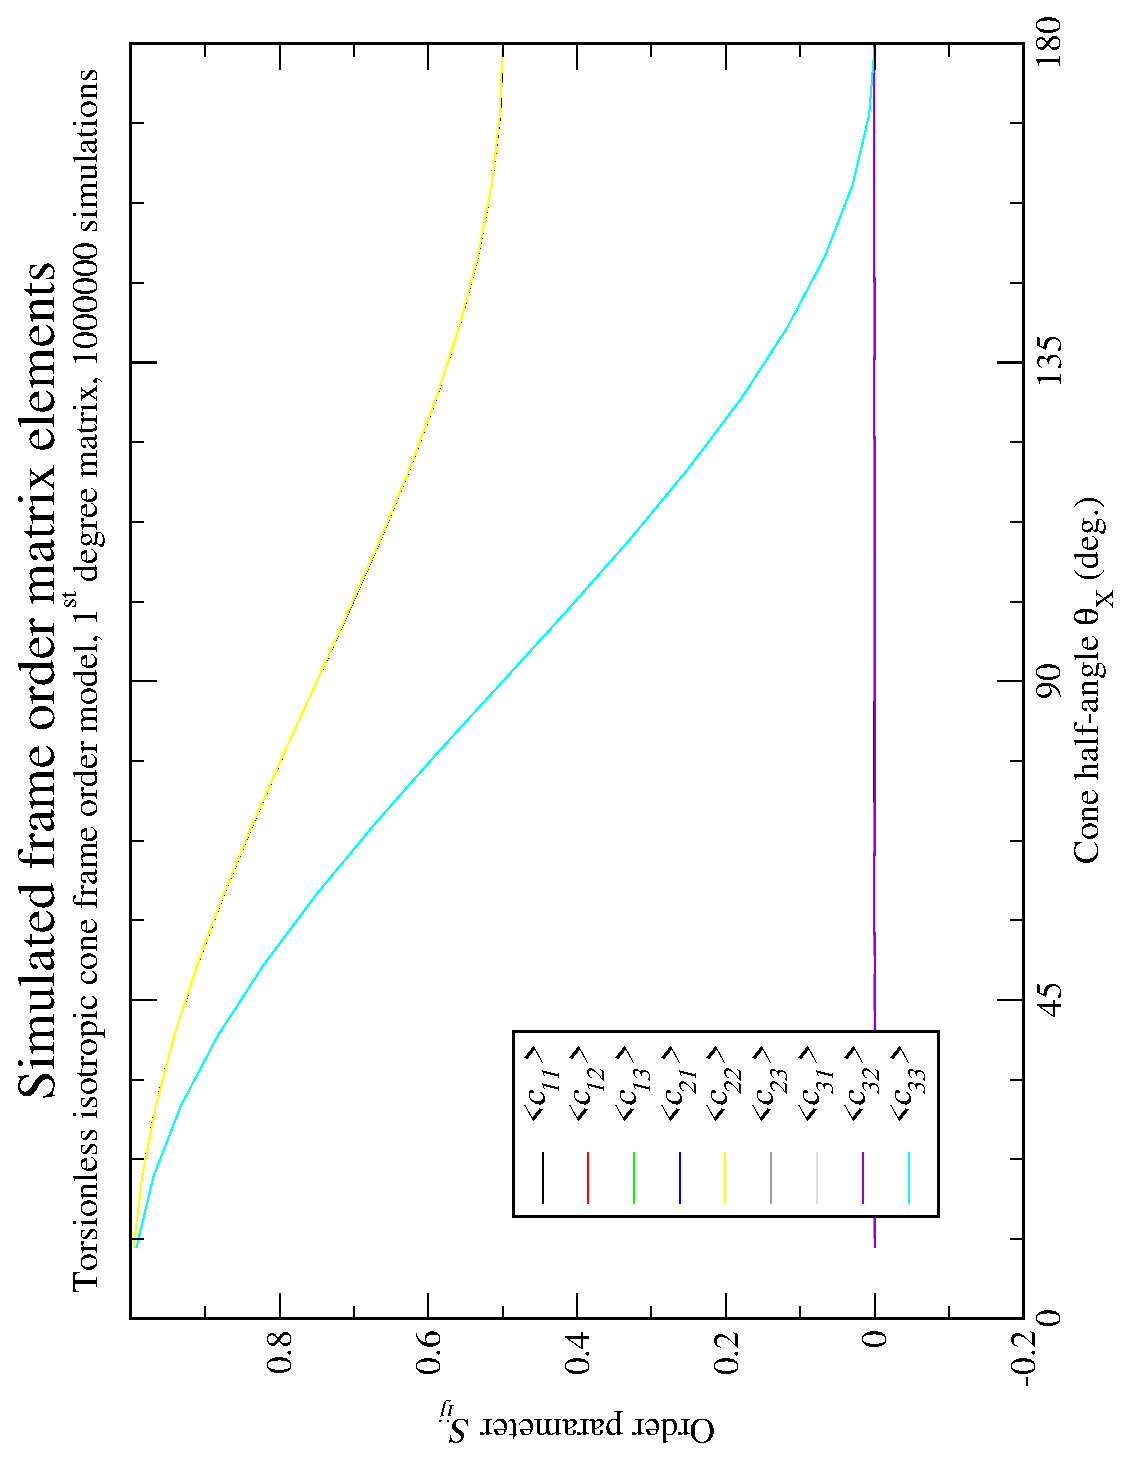
\includegraphics[width=.5\textwidth]{images/frame_order_matrix/Sij_iso_cone_torsionless_in_frame_theta_x_ens1000000.eps} &
    \includegraphics[width=.5\textwidth]{images/frame_order_matrix/Sij_iso_cone_torsionless_in_frame_theta_x_calc.eps} \\
    \\[-5pt]
    \includegraphics[width=.5\textwidth]{images/frame_order_matrix/Sijkl_iso_cone_torsionless_in_frame_theta_x_ens1000000.eps} &
    \includegraphics[width=.5\textwidth]{images/frame_order_matrix/Sijkl_iso_cone_torsionless_in_frame_theta_x_calc.eps} \\
  \end{tabular}
  \caption[Torsionless isotropic cone simulated and calculated in-frame Daeg$^{(1)}$ and Daeg$^{(2)}$ elements.]{
    The torsionless isotropic cone model simulated and calculated in-frame $\FOone$ and $\FOtwo$ frame order matrix elements.
    The top row corresponds to $\FOone$ and the bottom to $\FOtwo$.
    In these plots, $\theta_{\textrm{X}}$ corresponds to the cone opening half-angle $\conetheta$.
    Frame order matrix values have been calculated every 10 degrees.
  }
  \label{fig: simulated and calculated in-frame 1st and 2nd degree iso cone, torsionless frame order}
\end{figure}

\begin{figure}
\centering
  \begin{tabular}{@{}cc@{}}
    \includegraphics[width=.5\textwidth]{images/frame_order_matrix/Sij_iso_cone_torsionless_out_of_frame_theta_x_ens1000000.eps} &
    \includegraphics[width=.5\textwidth]{images/frame_order_matrix/Sij_iso_cone_torsionless_out_of_frame_theta_x_calc.eps} \\
    \\[-5pt]
    \includegraphics[width=.5\textwidth]{images/frame_order_matrix/Sijkl_iso_cone_torsionless_out_of_frame_theta_x_ens1000000.eps} &
    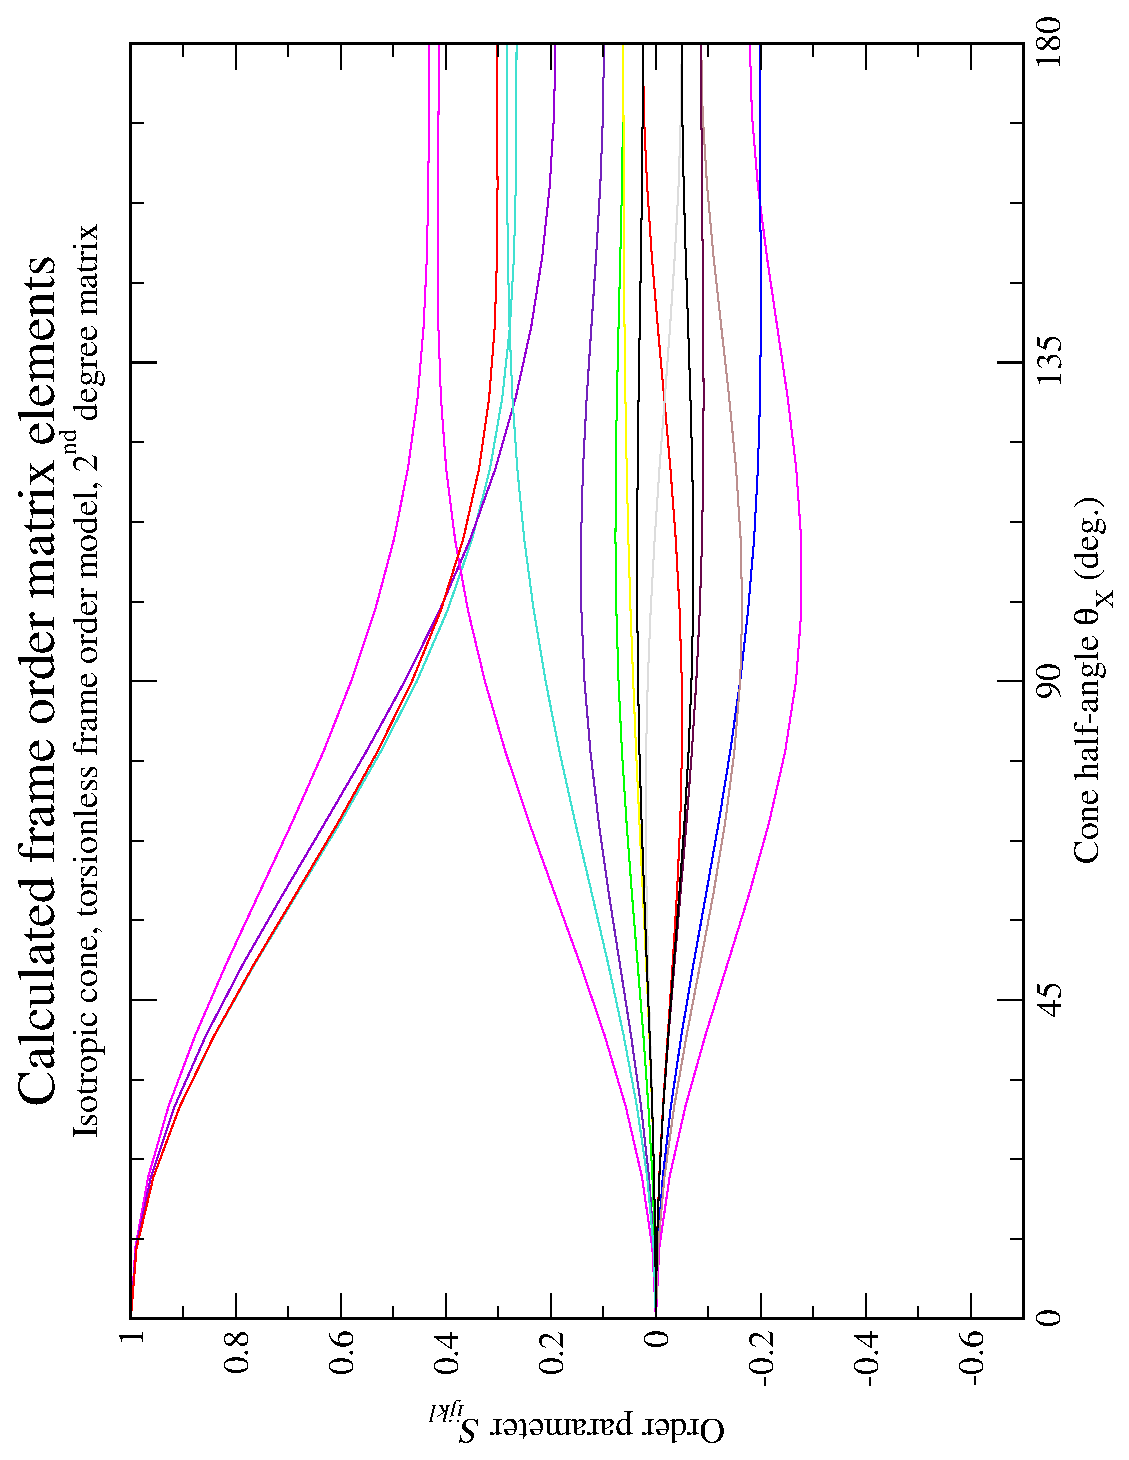
\includegraphics[width=.5\textwidth]{images/frame_order_matrix/Sijkl_iso_cone_torsionless_out_of_frame_theta_x_calc.eps} \\
  \end{tabular}
  \caption[Torsionless isotropic cone simulated and calculated out-of-frame Daeg$^{(1)}$ and Daeg$^{(2)}$ elements.]{
    The torsionless isotropic cone model simulated and calculated out-of-frame $\FOone$ and $\FOtwo$ frame order matrix elements.
    The top row corresponds to $\FOone$ and the bottom to $\FOtwo$.
    In these plots, $\theta_{\textrm{X}}$ corresponds to the cone opening half-angle $\conetheta$.
    Frame order matrix values have been calculated every 10 degrees.
  }
  \label{fig: simulated and calculated out-of-frame 1st and 2nd degree iso cone, torsionless frame order}
\end{figure}


\subsubsection{Torsionless isotropic cone rotation matrices}

The torsionless rotation matrix is defined in equation~\ref{eq: R matrix torsionless}.


\subsubsection{Torsionless isotropic cone frame order matrix}
\index{Frame order!matrix}

The frame order matrix is
\begin{subequations}
\begin{align}
    \FOn &= \left. \int_S R^{\otimes n} \diff S \right / \int_S \diff S , \\
         &= \left. \int_{-\pi}^{\pi} \int_{0}^{\conethetamax} R^{\otimes n} \sin\theta \diff\theta \diff\phi  \right / \int_S \diff S .
\end{align}
\end{subequations}

The surface normalisation factor is
\begin{subequations}
\begin{align}
    \int_S \diff S &= \int_{-\pi}^{\pi} \int_{0}^{\conethetamax} \sin\theta \diff\theta \diff\phi , \\
                   &= \int_{-\pi}^{\pi} \left( 1 - \cos\conethetamax \right) \diff\phi , \\
                   &= 2\pi \left( 1 - \cos\conethetamax \right) .
\end{align}
\end{subequations}


\paragraph{Torsionless isotropic cone \nth{1} degree frame order}

The \nth{1} degree frame order matrix with tensor rank-2 is
\begin{subequations} \label{eq: iso cone, torsionless 1st degree frame order matrix}
\begin{align}
    \FOone &= \left. \int_S R^{\otimes 1} \diff S \right / \int_S \diff S , \\
           &= \left. \int_S R \diff S \right / 2\pi \left( 1 - \cos\conethetamax \right) , \\
           &= \quart \begin{pmatrix}
                  \cos\conethetamax + 3 & .                     & . \\
                  .                     & \cos\conethetamax + 3 & . \\
                  .                     & .                     & 2\left( \cos\conethetamax + 1 \right) \\
              \end{pmatrix} .
\end{align}
\end{subequations}


\paragraph{Torsionless isotropic cone \nth{2} degree frame order}

The \nth{2} degree frame order matrix with tensor rank-4 consists of the following elements, using Kronecker product double indices from 0 to 8
\begin{subequations}
\begin{align}
    &\FO_{00} = \tfrac{1}{24} \left( 3\cos^2\conethetamax + 6\cos\conethetamax + 15 \right), \\
    &\FO_{11} = \tfrac{1}{24} \left( \cos^2\conethetamax + 10\cos\conethetamax + 13 \right) , \\
    &\FO_{22} = \tfrac{1}{24} \left( 4\cos^2\conethetamax + 10\cos\conethetamax + 10 \right) , \\
    &\FO_{33} = \FO_{11} , \\
    &\FO_{44} = \FO_{00} , \\
    &\FO_{55} = \FO_{22} , \\
    &\FO_{66} = \FO_{22} , \\
    &\FO_{77} = \FO_{22} , \\
    &\FO_{88} = \tfrac{1}{3} \left( \cos^2\conethetamax + \cos\conethetamax + 1 \right), \\
    &\FO_{04} = \tfrac{1}{24} \left( \cos^2\conethetamax - 2\cos\conethetamax + 1 \right) , \\
    &\FO_{40} = \FO_{04} , \\
    &\FO_{08} = -\tfrac{1}{6} \left( \cos^2\conethetamax + \cos\conethetamax - 2 \right) , \\
    &\FO_{80} = \FO_{08} , \\
    &\FO_{48} = \FO_{08} , \\
    &\FO_{84} = \FO_{08} , \\
    &\FO_{13} = \FO_{04} , \\
    &\FO_{31} = \FO_{04} , \\
    &\FO_{26} = -\FO_{08} , \\
    &\FO_{62} = -\FO_{08} , \\
    &\FO_{57} = -\FO_{08} , \\
    &\FO_{75} = -\FO_{08} .
\end{align}
\end{subequations}

After factorisation, the equations are
\begin{subequations} \label{eq: iso cone, torsionless 2nd degree frame order matrix}
\begin{align}
    &\FO_{00} = \tfrac{1}{8} \left( \cos\conethetamax + 1 \right)^2 + \half, \\
    &\FO_{11} = \tfrac{1}{24} \left( \cos\conethetamax + 5 \right)^2 - \half, \\
    &\FO_{22} = \tfrac{1}{96} \left( \left( 4\cos\conethetamax + 5 \right)^2 + 15 \right) , \\
    &\FO_{33} = \FO_{11} , \\
    &\FO_{44} = \FO_{00} , \\
    &\FO_{55} = \FO_{22} , \\
    &\FO_{66} = \FO_{22} , \\
    &\FO_{77} = \FO_{22} , \\
    &\FO_{88} = \tfrac{1}{12} \left( 2\cos\conethetamax + 1 \right)^2 + \quart, \\
    &\FO_{04} = \tfrac{1}{24} \left( \cos\conethetamax - 1 \right)^2 , \\
    &\FO_{40} = \FO_{04} , \\
    &\FO_{08} = -\tfrac{1}{6} \left( \cos\conethetamax + 2 \right) \left( \cos\conethetamax - 1 \right) , \\
    &\FO_{80} = \FO_{08} , \\
    &\FO_{48} = \FO_{08} , \\
    &\FO_{84} = \FO_{08} , \\
    &\FO_{13} = \FO_{04} , \\
    &\FO_{31} = \FO_{04} , \\
    &\FO_{26} = -\FO_{08} , \\
    &\FO_{62} = -\FO_{08} , \\
    &\FO_{57} = -\FO_{08} , \\
    &\FO_{75} = -\FO_{08} .
\end{align}
\end{subequations}

\subparagraph[Frame order matrix simulation and calculation]{Torsionless isotropic cone frame order matrix simulation and calculation}

The frame order matrix element simulation script from Section~\ref{sect: frame order simulation}, page~\pageref{sect: frame order simulation} was used to compare the implementation of equations~\ref{eq: iso cone, torsionless 1st degree frame order matrix} and~\ref{eq: iso cone, torsionless 2nd degree frame order matrix} above.
Frame order matrix $\FOone$ and $\FOtwo$ values were both simulated and calculated, both within and out of the motional eigenframe.
The in-frame $\FOone$ and $\FOtwo$ values are shown in figure~\ref{fig: simulated and calculated in-frame 1st and 2nd degree iso cone, torsionless frame order}.
The out-of-frame $\FOone$ and $\FOtwo$ values are shown in figure~\ref{fig: simulated and calculated out-of-frame 1st and 2nd degree iso cone, torsionless frame order}.



% The free rotor isotropic cone model.
\section{Free rotor isotropic cone frame order model}
\index{Frame order!model!isotropic cone, free rotor|textbf}


% Free rotor isotropic cone model parameterisation.
\subsection{Free rotor isotropic cone parameterisation}

For the free rotor variation of the isotropic cone model, the torsion angle restriction is absent and the model parameters are
\begin{subequations}
\begin{align}
    \Modelset &= \Posset + \Eigensetax + \Pivotsetone + \Orderset, \\
              &= \Possetfull + \Eigensetaxfull + \Pivotsetonefull + \left\{ \conethetamax \right\} ,
\end{align}
\end{subequations}

where $\aveposi$ are the average domain position translations and rotations, $\framei$ are the spherical angles defining the cone axis, $\pivoti$ are the coordinates of the pivot point, and $\conethetamax$ is the maximum cone opening half-angle.


% Free rotor isotropic cone model equations.
\subsection{Free rotor isotropic cone equations}

\begin{figure}
\centering
  \begin{tabular}{@{}cc@{}}
    \includegraphics[width=.5\textwidth]{images/frame_order_matrix/Sij_iso_cone_free_rotor_in_frame_theta_x_ens1000000.eps} &
    \includegraphics[width=.5\textwidth]{images/frame_order_matrix/Sij_iso_cone_free_rotor_in_frame_theta_x_calc.eps} \\
    \\[-5pt]
    \includegraphics[width=.5\textwidth]{images/frame_order_matrix/Sijkl_iso_cone_free_rotor_in_frame_theta_x_ens1000000.eps} &
    \includegraphics[width=.5\textwidth]{images/frame_order_matrix/Sijkl_iso_cone_free_rotor_in_frame_theta_x_calc.eps} \\
  \end{tabular}
  \caption[Free-rotor isotropic cone simulated and calculated in-frame Daeg$^{(1)}$ and Daeg$^{(2)}$ elements.]{
    The free rotor isotropic cone model simulated and calculated in-frame $\FOone$ and $\FOtwo$ frame order matrix elements.
    The top row corresponds to $\FOone$ and the bottom to $\FOtwo$.
    In these plots, $\theta_{\textrm{X}}$ corresponds to the cone opening half-angle $\conetheta$.
    Frame order matrix values have been calculated every 10 degrees.
  }
  \label{fig: simulated and calculated in-frame 1st and 2nd degree iso cone, free rotor frame order}
\end{figure}

\begin{figure}
\centering
  \begin{tabular}{@{}cc@{}}
    \includegraphics[width=.5\textwidth]{images/frame_order_matrix/Sij_iso_cone_free_rotor_out_of_frame_theta_x_ens1000000.eps} &
    \includegraphics[width=.5\textwidth]{images/frame_order_matrix/Sij_iso_cone_free_rotor_out_of_frame_theta_x_calc.eps} \\
    \\[-5pt]
    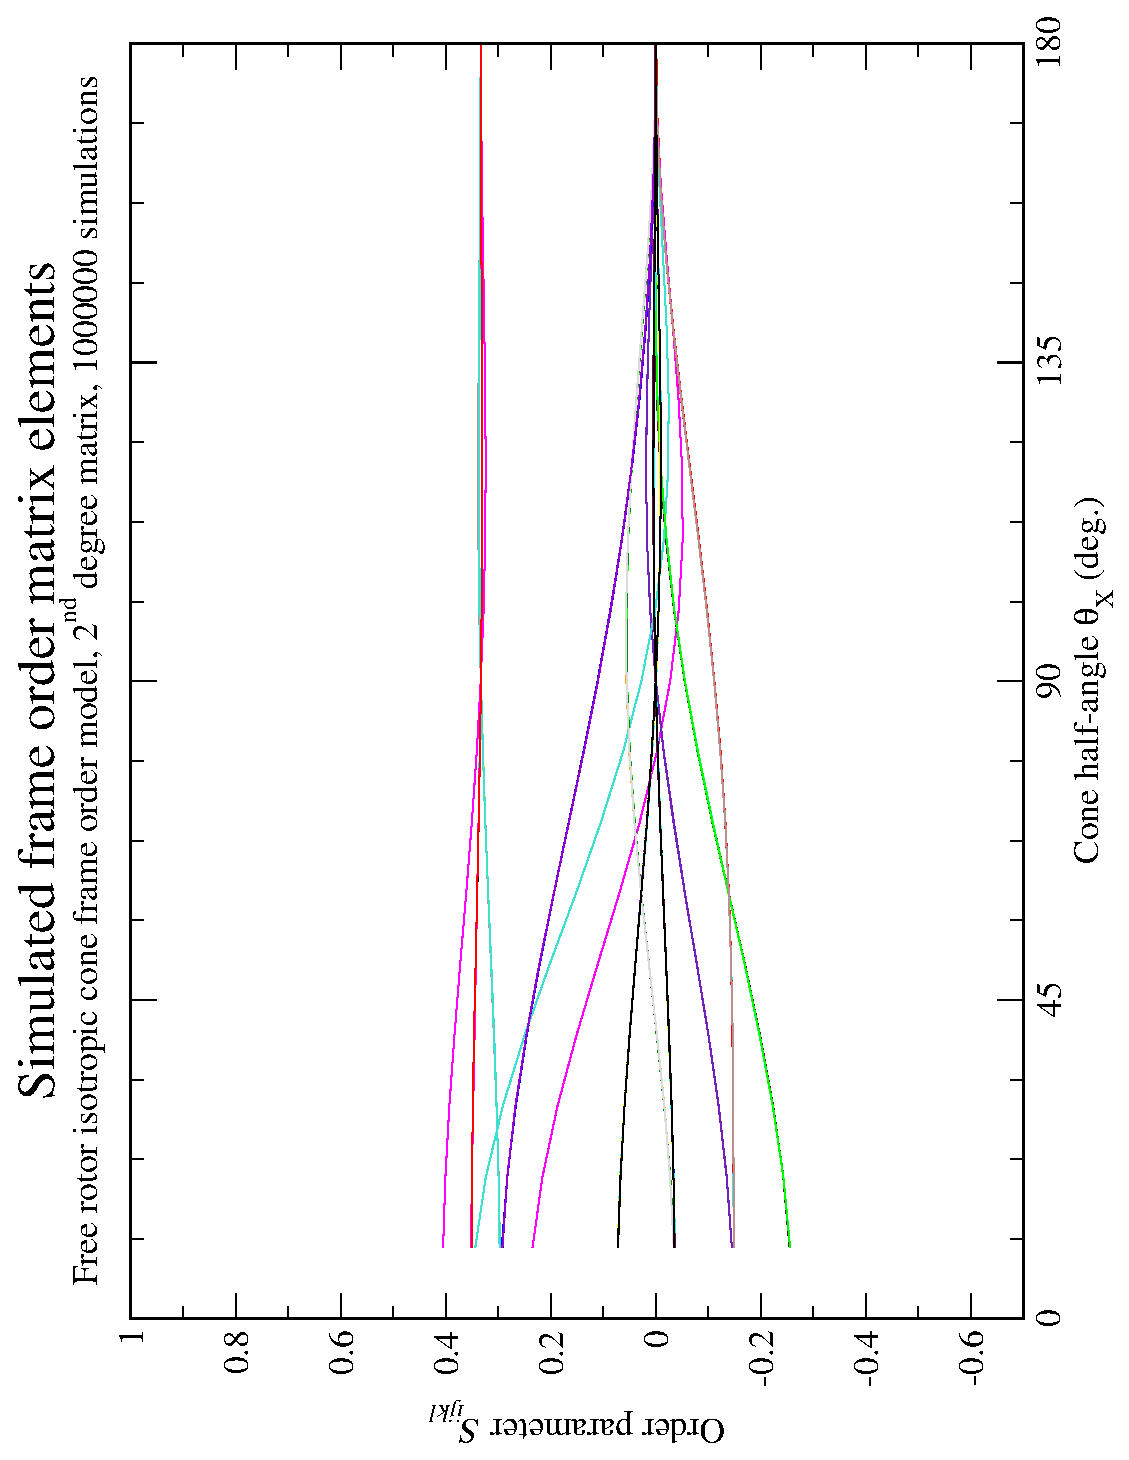
\includegraphics[width=.5\textwidth]{images/frame_order_matrix/Sijkl_iso_cone_free_rotor_out_of_frame_theta_x_ens1000000.eps} &
    \includegraphics[width=.5\textwidth]{images/frame_order_matrix/Sijkl_iso_cone_free_rotor_out_of_frame_theta_x_calc.eps} \\
  \end{tabular}
  \caption[Free-rotor isotropic cone simulated and calculated out-of-frame Daeg$^{(1)}$ and Daeg$^{(2)}$ elements.]{
    The free rotor isotropic cone model simulated and calculated out-of-frame $\FOone$ and $\FOtwo$ frame order matrix elements.
    The top row corresponds to $\FOone$ and the bottom to $\FOtwo$.
    In these plots, $\theta_{\textrm{X}}$ corresponds to the cone opening half-angle $\conetheta$.
    Frame order matrix values have been calculated every 10 degrees.
  }
  \label{fig: simulated and calculated out-of-frame 1st and 2nd degree iso cone, free rotor frame order}
\end{figure}


\subsubsection{Free rotor isotropic cone rotation matrices}

The rotation matrix is the full torsion-tilt rotation matrix of equation~\ref{eq: R torsion-tilt} on page~\pageref{eq: R torsion-tilt}.

\subsubsection{Free rotor isotropic cone frame order matrix}
\index{Frame order!matrix}

The frame order matrix is
\begin{subequations}
\begin{align}
    \FOn &= \left. \int_S R^{\otimes n} \diff S \right / \int_S \diff S , \\
         &= \left. \int_{-\pi}^{\pi} \int_{-\pi}^{\pi} \int_{0}^{\conethetamax} R^{\otimes n} \sin\theta \diff\theta \diff\phi \diff\sigma  \right / \int_S \diff S .
\end{align}
\end{subequations}

The surface normalisation factor is
\begin{subequations}
\begin{align}
    \int_S \diff S &= \int_{-\pi}^{\pi} \int_{-\pi}^{\pi} \int_{0}^{\conethetamax} \sin\theta \diff\theta \diff\phi \diff\sigma , \\
                   &= \int_{-\pi}^{\pi} \int_{-\pi}^{\pi} \left( 1 - \cos\conethetamax \right) \diff\phi \diff\sigma , \\
                   &= \int_{-\pi}^{\pi} 2\pi \left( 1 - \cos\conethetamax \right) \diff\sigma , \\
                   &= 4\pi^2 \left( 1 - \cos\conethetamax \right) .
\end{align}
\end{subequations}


\paragraph{Free rotor isotropic cone \nth{1} degree frame order}

The \nth{1} degree frame order matrix with tensor rank-2 is
\begin{subequations} \label{eq: iso cone, free rotor 1st degree frame order matrix}
\begin{align}
    \FOone &= \left. \int_S R^{\otimes 1} \diff S \right / \int_S \diff S , \\
           &= \left. \int_S R \diff S \right / 2\pi \left( 1 - \cos\conethetamax \right) , \\
           &= \half \begin{pmatrix}
                  . & . & . \\
                  . & . & . \\
                  . & . & \cos\conethetamax + 1 \\
              \end{pmatrix} .
\end{align}
\end{subequations}


\paragraph{Free rotor isotropic cone \nth{2} degree frame order}


The \nth{2} degree frame order matrix with tensor rank-4 consists of the following elements, using Kronecker product double indices from 0 to 8
\begin{subequations} \label{eq: iso cone, free rotor 2nd degree frame order matrix}
\begin{align}
    &\FO_{00} = \tfrac{1}{12} \left( \cos^2\conethetamax + \cos\conethetamax + 4 \right) , \\
    &\FO_{11} = \tfrac{1}{4} \left( \cos\conethetamax + 1 \right) , \\
    &\FO_{22} = 0 , \\
    &\FO_{33} = \FO_{11} , \\
    &\FO_{44} = \FO_{00} , \\
    &\FO_{55} = 0 , \\
    &\FO_{66} = 0 , \\
    &\FO_{77} = 0 , \\
    &\FO_{88} = \tfrac{1}{3} \left( \cos^2\conethetamax + \cos\conethetamax + 1 \right) , \\
    &\FO_{04} = \FO_{00} , \\
    &\FO_{40} = \FO_{00} , \\
    &\FO_{08} = -\tfrac{1}{6} \left( \cos^2\conethetamax + \cos\conethetamax - 2 \right) , \\
    &\FO_{80} = \FO_{08} , \\
    &\FO_{48} = \FO_{08} , \\
    &\FO_{84} = \FO_{08} , \\
    &\FO_{13} = -\FO_{11} , \\
    &\FO_{31} = -\FO_{11} , \\
    &\FO_{26} = 0 , \\
    &\FO_{62} = 0 , \\
    &\FO_{57} = 0 , \\
    &\FO_{75} = 0 .
\end{align}
\end{subequations}


\subparagraph[Frame order matrix simulation and calculation]{Free rotor isotropic cone frame order matrix simulation and calculation}

The frame order matrix element simulation script from Section~\ref{sect: frame order simulation}, page~\pageref{sect: frame order simulation} was used to compare the implementation of equations~\ref{eq: iso cone, free rotor 1st degree frame order matrix} and~\ref{eq: iso cone, free rotor 2nd degree frame order matrix} above.
Frame order matrix $\FOone$ and $\FOtwo$ values were both simulated and calculated, both within and out of the motional eigenframe.
The in-frame $\FOone$ and $\FOtwo$ values are shown in figure~\ref{fig: simulated and calculated in-frame 1st and 2nd degree iso cone, free rotor frame order}.
The out-of-frame $\FOone$ and $\FOtwo$ values are shown in figure~\ref{fig: simulated and calculated out-of-frame 1st and 2nd degree iso cone, free rotor frame order}.




% The pseudo-ellipse model.
%~~~~~~~~~~~~~~~~~~~~~~~~~~

\section{Pseudo-ellipse frame order model}
\index{Frame order!model!pseudo-ellipse|textbf}




% Pseudo-ellipse model parameterisation.
%~~~~~~~~~~~~~~~~~~~~~~~~~~~~~~~~~~~~~~~

\subsection{Pseudo-ellipse parameterisation}

To extend to the next level of motional complexity above the isotropic cone models, an anisotropic cone can be modelled.
This cone is defined via the ball and socket joint pivoted mechanics with an angular restriction in all three angles.
The simplest anisotropic distribution would be to create an ellipse using the standard quadric surface formula for an elliptic cone
\begin{equation}
    \frac{x^2}{a^2} + \frac{y^2}{b^2} - \frac{z^2}{c^2} = 0 .
\end{equation}

Let the two cone opening half-angles of the ellipse be $\conethetax$ and $\conethetay$.
For a sphere of radius $z = 1$ and using the tilt angles $\conetheta$ and $\phi$, a boundary polar angle $\conethetamax$ can be modelled as
\begin{equation} \label{eq: pseudo-ellipse}
    \frac{1}{\conethetamax^2} = \frac{\cos^2\phi}{\conethetax^2} + \frac{\sin^2\phi}{\conethetay^2} .
\end{equation}

As the quadric constants $a$, $b$ and $c$ are angles rather than axis lengths, this is not a true ellipse.
It will therefore instead be called a pseudo-ellipse.
The form of this pseudo-elliptic cone is shown in figure~\ref{fig: pseudo-elliptic cone}.

% The pseudo-elliptic cone figure.
% This is from frame_order/aniso_distributions/pseudo_elliptic2/.
\begin{figure}
  \centerline{
    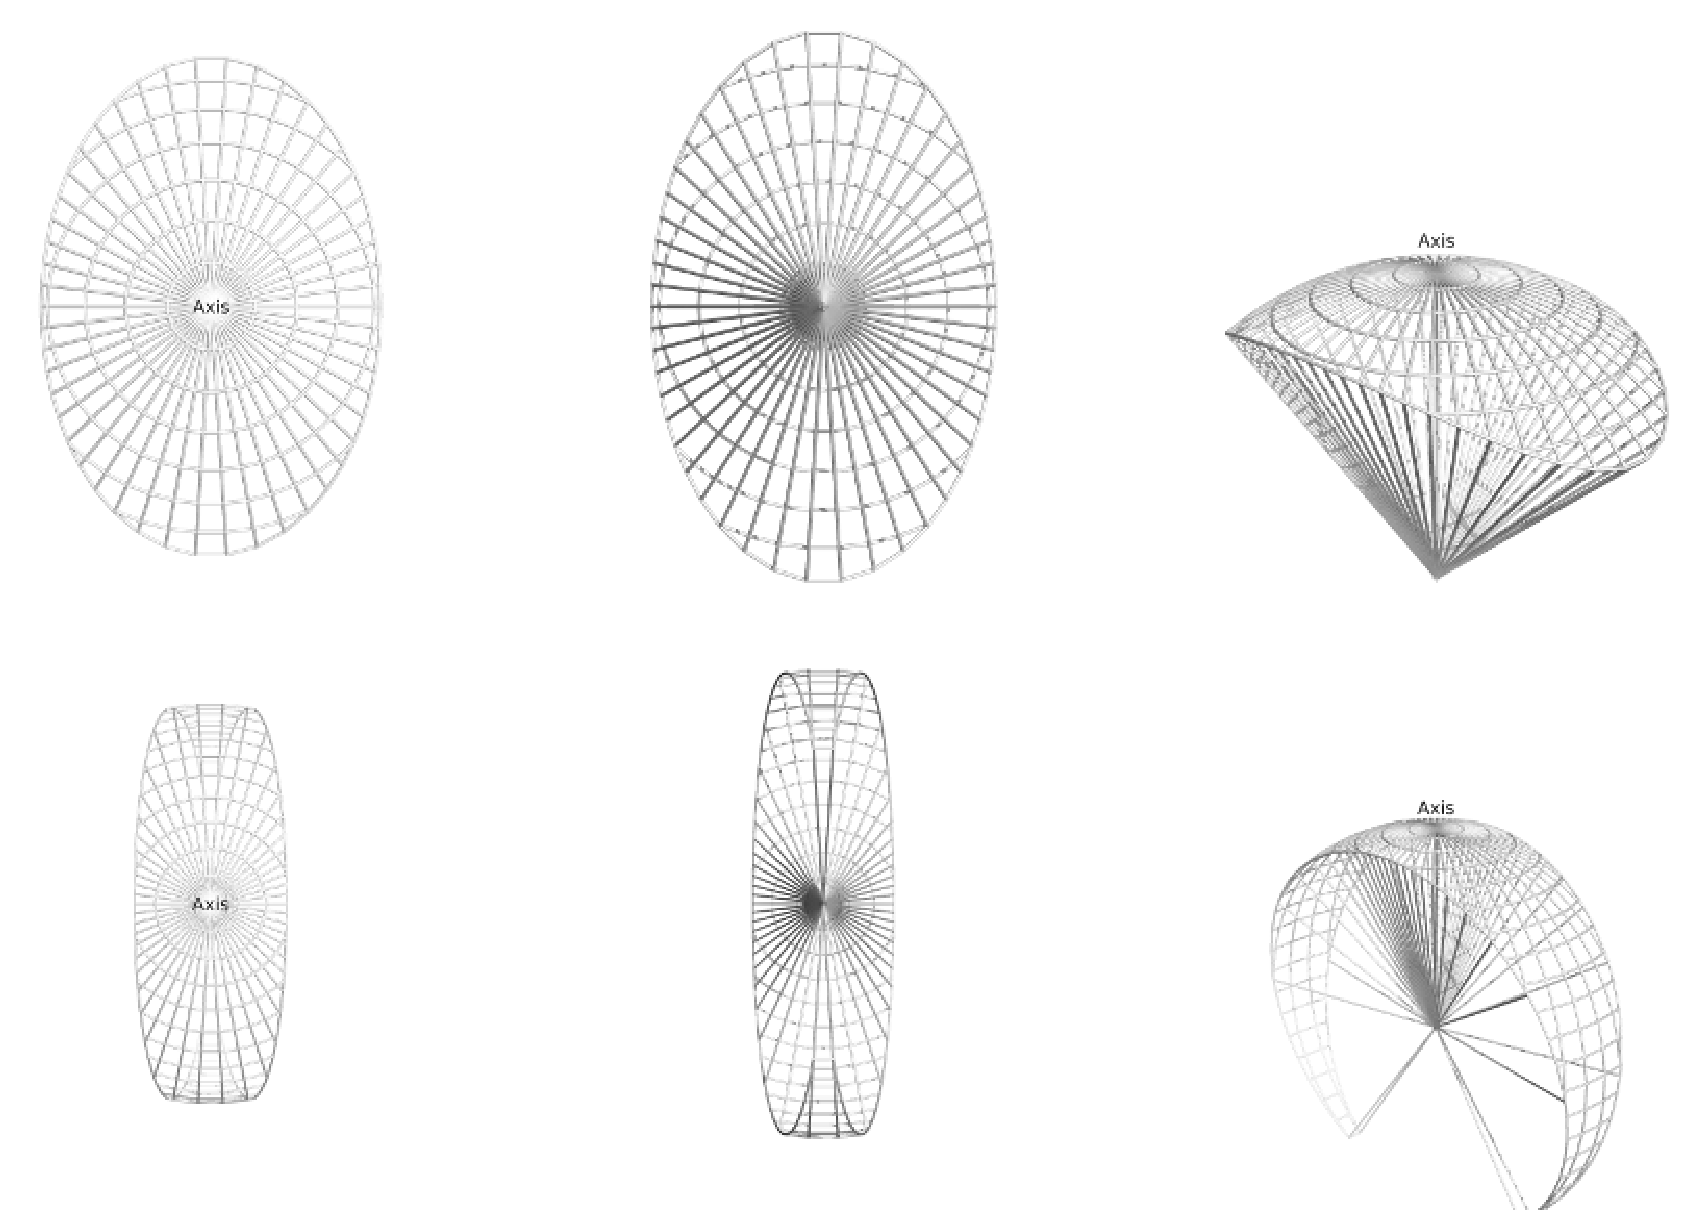
\includegraphics[width=0.7\textwidth]{images/pseudo_elliptic_cone}
  }
  \caption[The pseudo-elliptic cone.]{
      The pseudo-elliptic cone.
      The top three representations are for $\conethetax = 30^\circ$ and $\conethetay = 50^\circ$.
      The bottom three representations are for $\conethetax = 20^\circ$ and $\conethetay = 160^\circ$.
  }
  \label{fig: pseudo-elliptic cone}
\end{figure}


The model consists of the average domain position, a single pivot point, the full motional eigenframe, and the maximum cone opening and torsion half-angles
\begin{subequations}
\begin{align}
    \Modelset &= \Posset + \Eigenset + \Pivotsetone + \Orderset, \\
              &= \Possetfull + \Eigensetfull + \Pivotsetonefull + \left\{ \conethetax, \conethetay, \conesmax \right\} ,
\end{align}
\end{subequations}

where $\aveposi$ are the average domain position translations and rotations, $\framei$ are the Euler angles defining the motional eigenframe, $\pivoti$ are the coordinates of the pivot point, $\conethetax$ and $\conethetay$ are the maximum cone opening half-angles, and $\conesmax$ is the torsion half-angle.



% Pseudo-elliptic cosine 2D trigonometric function.
%~~~~~~~~~~~~~~~~~~~~~~~~~~~~~~~~~~~~~~~~~~~~~~~~~~

\subsection{Derivation of a 2D trigonometric function - the pseudo-elliptic cosine}

For the surface normalisation factor of the pseudo-elliptic cone, the integral from equation~\ref{eq: pseudo-ellipse surface norm non-integratable} on page~\pageref{eq: pseudo-ellipse surface norm non-integratable} is
\begin{equation}
    \int_S \diff S = \int_{-\conesmax}^{\conesmax} \int_{-\pi}^{\pi} \left( 1 - \cos\conethetamax \right) \diff\phi \diff\sigma .
\end{equation}

When combined with the pseudo-ellipse of equation~\ref{eq: pseudo-ellipse}, this becomes the intractable integral
\begin{equation}
    \int_S \diff S = \bigintsss_{-\conesmax}^{\conesmax} \bigintsss_{-\pi}^{\pi} \left( 1 - \cos \left( \frac{1}{\sqrt{\frac{\cos^2\phi}{\conethetax^2} + \frac{\sin^2\phi}{\conethetay^2}}} \right) \right) \diff\phi \diff\sigma ,
\end{equation}

Instead the cosine series expansion will be used
\begin{align}
    \cos \conethetamax &= 1 - \frac{{\conethetamax}^2}{2!} + \frac{{\conethetamax}^4}{4!} - \frac{{\conethetamax}^6}{6!} + \frac{{\conethetamax}^8}{8!} - \frac{{\conethetamax}^{10}}{10!} + \cdots , \\
                       &= \sum_{n=0}^\infty \frac{(-1)^n}{(2n)!} {\conethetamax}^{2n} .
\end{align}

Integrating each element of the sum over the $\phi$ parameter and using the assumption that $\conethetax, \conethetay \ge 0$ gives
\begin{gather}
    \int_{-\pi}^{\pi} \frac{{\conethetamax}^2}{2!} \diff\phi = \pi \conethetax \conethetay , \nonumber \\
    \int_{-\pi}^{\pi} \frac{{\conethetamax}^4}{4!} \diff\phi = \frac{\pi \conethetax \conethetay}{24} \left( \conethetax ^2 + \conethetay^2 \right) , \nonumber \\
    \int_{-\pi}^{\pi} \frac{{\conethetamax}^6}{6!} \diff\phi = \frac{\pi \conethetax \conethetay}{2880} \left( 3\conethetax ^4 + 2\conethetax ^2\conethetay^2 + 3\conethetay^4 \right) , \nonumber \\
    \int_{-\pi}^{\pi} \frac{{\conethetamax}^8}{8!} \diff\phi = \frac{\pi \conethetax \conethetay}{322560} \left( 5\conethetax ^6 + 3\conethetax ^4\conethetay^2 + 3\conethetax ^2\conethetay^4 + 5\conethetay^6 \right) , \nonumber \\
    \int_{-\pi}^{\pi} \frac{{\conethetamax}^{10}}{10!} \diff\phi = \frac{\pi \conethetax \conethetay}{232243200} \left( 35\conethetax ^8 + 20\conethetax ^6\conethetay^2 + 18\conethetax ^4\conethetay^4 + 20x^2\conethetay^6 + 35\conethetay^8 \right) , \nonumber \\
    \dots
\end{gather}

Therefore a new two dimension trigonometric function, the pseudo-elliptic cosine, can be defined as
\begin{subequations}
\begin{align}
    \pec(\conethetax, \conethetay)
        &= \int_{-\pi}^{\pi} \left( 1 - \cos\conethetamax \right) \diff\phi , \\
        &= 2\pi \conethetax \conethetay \sum_{n=0}^\infty \frac{(-1)^n}{4^n(2n+2)!} f_n(\conethetax, \conethetay) .
\end{align}
\end{subequations}

Let
\begin{align}
    a = \conethetax^2, \nonumber \\
    b = \conethetay^2,
\end{align}

then the first of the $f_n(\conethetax, \conethetay)$ equations are
\begin{gather}
    f_0 = 1 , \nonumber \\
    f_1 = 2a + 2b , \nonumber \\
    f_2 = 6a^2 + 4ab + 6b^2 , \nonumber \\
    f_3 = 20a^3 + 12a^2b + 12ab^2 + 20b^3 , \nonumber \\
    f_4 = 70a^4 + 40a^3b + 36a^2b^2 + 40ab^3 + 70b^4 , \nonumber \\
    f_5 = 252a^5 + 140a^4b + 120a^3b^2 + 120a^2b^3 + 140ab^4 + 252b^5 , \nonumber \\
    f_6 = 924a^6 + 504a^5b + 420a^4b^2 + 400a^3b^3 + 420a^2b^4 + 504ab^5 + 924b^6 , \nonumber \\
    f_7 = 3432a^7 + 1848a^6b + 1512a^5b^2 + 1400a^4b^3 + 1400a^3b^4 + 1512a^2b^5 + 1848ab^6 + 3432b^7 , \nonumber \\
    \dots
\end{gather}

Or
\begin{footnotesize}
\begin{gather}
    f_0 = 1 , \nonumber \\
    f_1 = 2(a + b) , \nonumber \\
    f_2 = 6(a^2 + b^2) + 4ab , \nonumber \\
    f_3 = 20(a^3 + b^3) + 12(a^2b + ab^2) , \nonumber \\
    f_4 = 70(a^4 + b^4) + 40(a^3b + ab^3) + 36a^2b^2 , \nonumber \\
    f_5 = 252(a^5 + b^5) + 140(a^4b + ab^4) + 120(a^3b^2 + a^2b^3) , \nonumber \\
    f_6 = 924(a^6 + b^6) + 504(a^5b + ab^5) + 420(a^4b^2 + a^2b^4) + 400a^3b^3 , \nonumber \\
    f_7 = 3432(a^7 + b^7) + 1848(a^6b + ab^6) + 1512(a^5b^2 + a^2b^5) + 1400(a^4b^3 + a^3b^4) , \nonumber \\
    f_8 = 12870(a^8 + b^8) + 6864(a^7b + ab^7) + 5544(a^6b^2 + a^2b^6) + 5040(a^5b^3 + a^3b^5) + 4900a^4b^4 , \nonumber \\
    f_9 = 48620(a^9 + b^9) + 25740(a^8b + ab^8) + 20592(a^7b^2 + a^2b^7) + 18480(a^6b^3 + a^3b^6) + 17640(a^5b^4 + a^4b^5) , \nonumber \\
    f_{10} = 184756(a^{10} + b^{10}) + 97240(a^9b + ab^9) + 77220(a^8b^2 + a^2b^8) + 68640(a^7b^3 + a^3b^7) + 64680(a^6b^4 + a^4b^6) + 63504a^5b^5 , \nonumber \\
    \dots
\end{gather}
\end{footnotesize}

This series expansion up to $n = 10$ is sufficient for writing a fast and accurate $\pec$ function implementation in computer code.
The numerical representation of this function is shown in figure~\ref{fig: pec function}.

% pec() figure.
% This is from frame_order/pec/.
\begin{figure}
\centering
  \begin{tabular}{@{}cc@{}}
    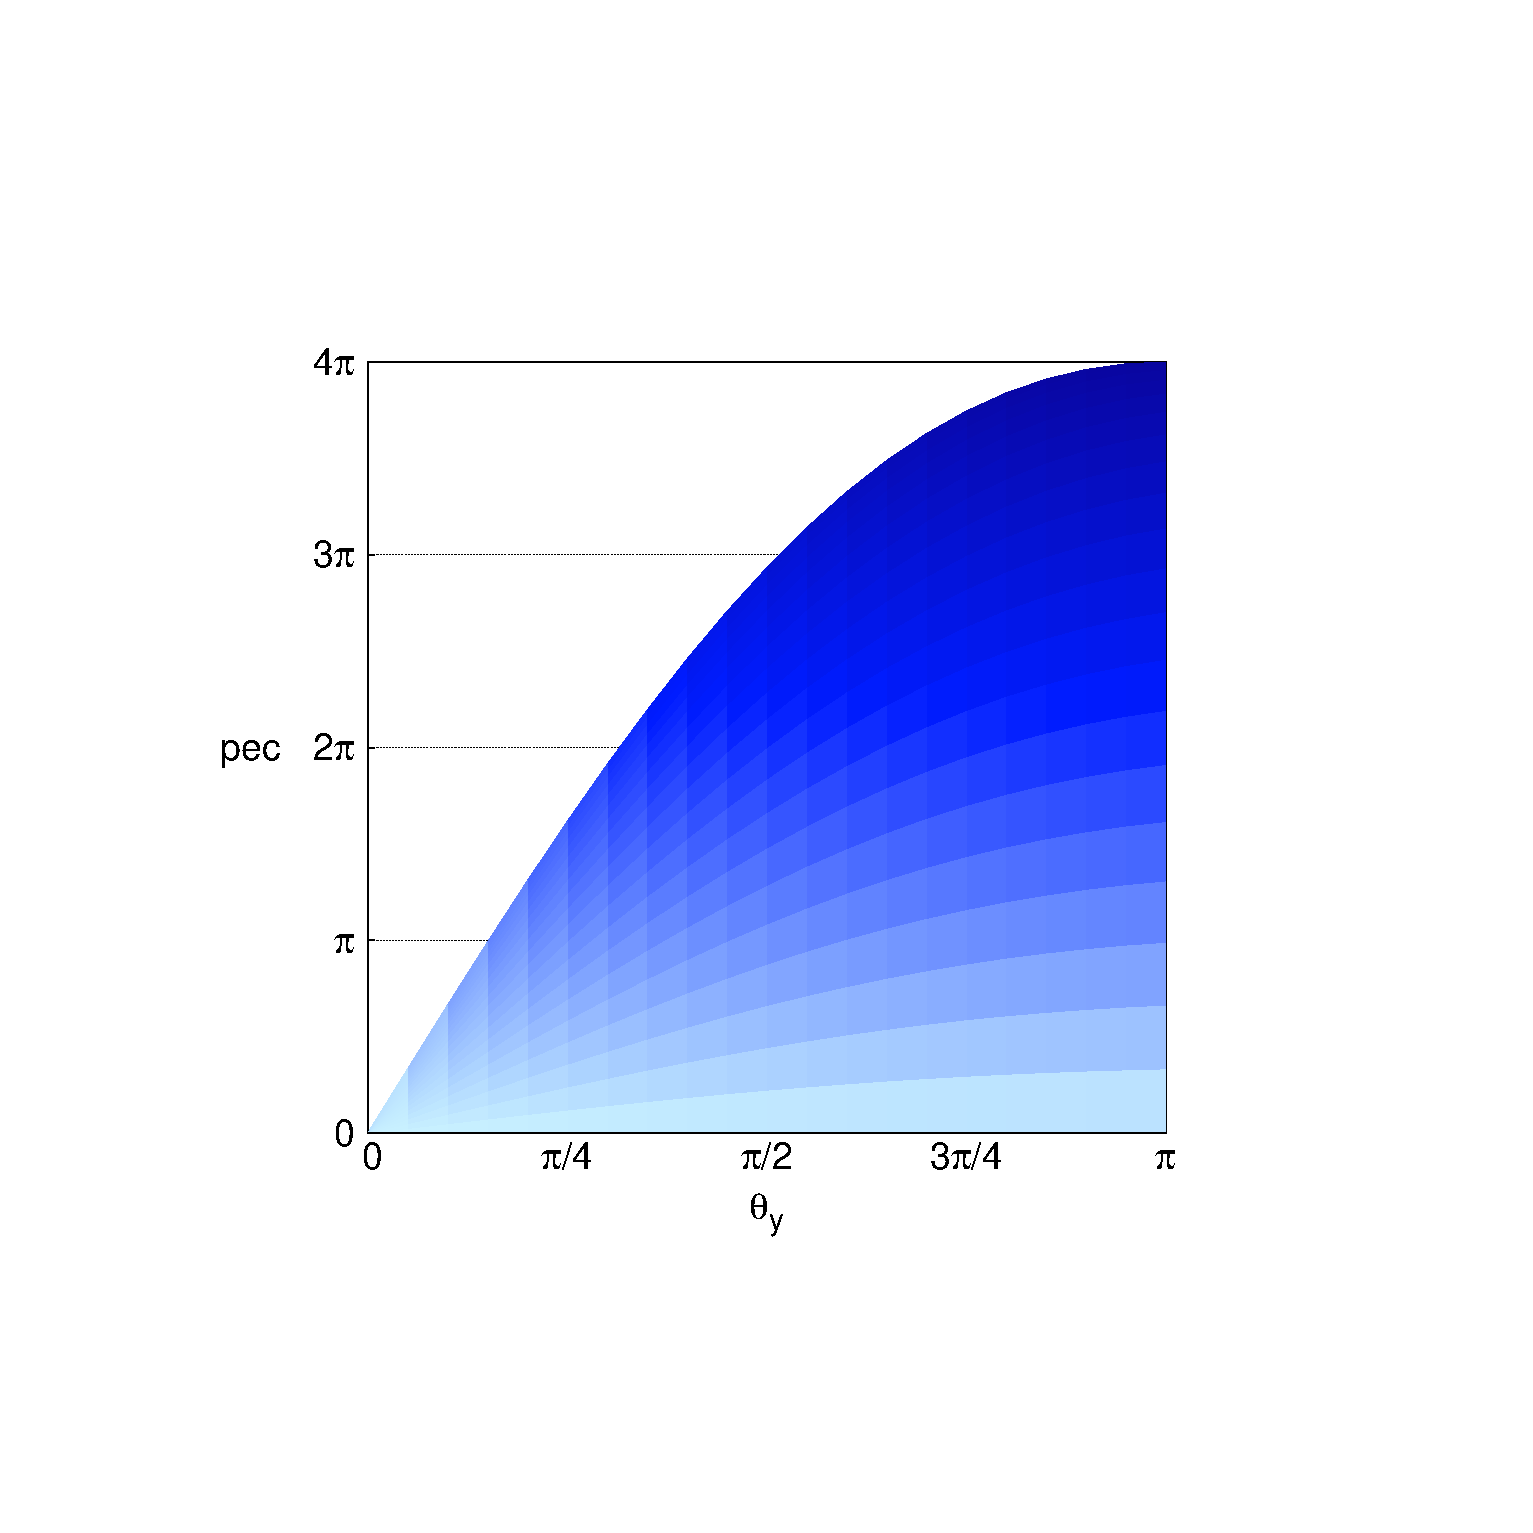
\includegraphics[width=.5\textwidth,bb=150 150 650 650]{images/pec_y.eps} &
    \includegraphics[width=.5\textwidth,bb=80 80 730 740]{images/pec_diag.eps}
  \end{tabular}
  \caption[Pseudo-ellipse cosine 2D trigonometric function.]{
    The pseudo-ellipse cosine 2D trigonometric function.
    This is the surface area on a unit sphere bounded by the pseudo-elliptic cone.
  }
  \label{fig: pec function}
\end{figure}



% Pseudo-ellipse model equations.
%--------------------------------

\subsection{Pseudo-ellipse equations}

\begin{figure}
\centering
  \begin{tabular}{@{}cc@{}}
    \includegraphics[width=.5\textwidth]{images/frame_order_matrix/Sij_pseudo-ellipse_in_frame_theta_x_ens1000000.eps} &
    \includegraphics[width=.5\textwidth]{images/frame_order_matrix/Sij_pseudo-ellipse_in_frame_theta_x_calc.eps} \\
    \\[-5pt]
    \includegraphics[width=.5\textwidth]{images/frame_order_matrix/Sij_pseudo-ellipse_in_frame_theta_y_ens1000000.eps} &
    \includegraphics[width=.5\textwidth]{images/frame_order_matrix/Sij_pseudo-ellipse_in_frame_theta_y_calc.eps} \\
    \\[-5pt]
    \includegraphics[width=.5\textwidth]{images/frame_order_matrix/Sij_pseudo-ellipse_in_frame_theta_z_ens1000000.eps} &
    \includegraphics[width=.5\textwidth]{images/frame_order_matrix/Sij_pseudo-ellipse_in_frame_theta_z_calc.eps} \\
  \end{tabular}
  \caption[Pseudo-ellipse simulated and calculated in-frame Daeg$^{(1)}$ elements.]{
    The pseudo-ellipse model simulated and calculated in-frame $\FOone$ frame order matrix elements.
    In these plots, $\theta_{\textrm{X}}$ corresponds to the cone opening half-angle $\conethetax$, $\theta_{\textrm{Y}}$ to the cone opening half-angle $\conethetay$ and $\theta_{\textrm{Z}}$ to torsion half-angle $\conesmax$.
    When the half-angle is not varied, the angle is fixed to either $\conethetax = \pi/4$, $\conethetay = 3\pi/8$ or $\conesmax = \pi/6$.
    Frame order matrix values have been calculated every 10 degrees.
    The first angle for the calculated $\theta_{\textrm{X}}$ and $\theta_{\textrm{Y}}$ graphs is set to 0.01 degrees as a pseudo-ellipse cone opening angle of 0.0 cannot be correctly handled by the numerical integration.
  }
  \label{fig: simulated and calculated in-frame 1st degree pseudo-ellipse frame order}
\end{figure}

\begin{figure}
\centering
  \begin{tabular}{@{}cc@{}}
    \includegraphics[width=.5\textwidth]{images/frame_order_matrix/Sijkl_pseudo-ellipse_in_frame_theta_x_ens1000000.eps} &
    \includegraphics[width=.5\textwidth]{images/frame_order_matrix/Sijkl_pseudo-ellipse_in_frame_theta_x_calc.eps} \\
    \\[-5pt]
    \includegraphics[width=.5\textwidth]{images/frame_order_matrix/Sijkl_pseudo-ellipse_in_frame_theta_y_ens1000000.eps} &
    \includegraphics[width=.5\textwidth]{images/frame_order_matrix/Sijkl_pseudo-ellipse_in_frame_theta_y_calc.eps} \\
    \\[-5pt]
    \includegraphics[width=.5\textwidth]{images/frame_order_matrix/Sijkl_pseudo-ellipse_in_frame_theta_z_ens1000000.eps} &
    \includegraphics[width=.5\textwidth]{images/frame_order_matrix/Sijkl_pseudo-ellipse_in_frame_theta_z_calc.eps} \\
  \end{tabular}
  \caption[Pseudo-ellipse simulated and calculated in-frame Daeg$^{(2)}$ elements.]{
    The pseudo-ellipse model simulated and calculated in-frame $\FOtwo$ frame order matrix elements.
    In these plots, $\theta_{\textrm{X}}$ corresponds to the cone opening half-angle $\conethetax$, $\theta_{\textrm{Y}}$ to the cone opening half-angle $\conethetay$ and $\theta_{\textrm{Z}}$ to torsion half-angle $\conesmax$.
    When the half-angle is not varied, the angle is fixed to either $\conethetax = \pi/4$, $\conethetay = 3\pi/8$ or $\conesmax = \pi/6$.
    Frame order matrix values have been calculated every 10 degrees.
    The first angle for the calculated $\theta_{\textrm{X}}$ and $\theta_{\textrm{Y}}$ graphs is set to 0.01 degrees as a pseudo-ellipse cone opening angle of 0.0 cannot be correctly handled by the numerical integration.
  }
  \label{fig: simulated and calculated in-frame 2nd degree pseudo-ellipse frame order}
\end{figure}

\begin{figure}
\centering
  \begin{tabular}{@{}cc@{}}
    \includegraphics[width=.5\textwidth]{images/frame_order_matrix/Sij_pseudo-ellipse_out_of_frame_theta_x_ens1000000.eps} &
    \includegraphics[width=.5\textwidth]{images/frame_order_matrix/Sij_pseudo-ellipse_out_of_frame_theta_x_calc.eps} \\
    \\[-5pt]
    \includegraphics[width=.5\textwidth]{images/frame_order_matrix/Sij_pseudo-ellipse_out_of_frame_theta_y_ens1000000.eps} &
    \includegraphics[width=.5\textwidth]{images/frame_order_matrix/Sij_pseudo-ellipse_out_of_frame_theta_y_calc.eps} \\
    \\[-5pt]
    \includegraphics[width=.5\textwidth]{images/frame_order_matrix/Sij_pseudo-ellipse_out_of_frame_theta_z_ens1000000.eps} &
    \includegraphics[width=.5\textwidth]{images/frame_order_matrix/Sij_pseudo-ellipse_out_of_frame_theta_z_calc.eps} \\
  \end{tabular}
  \caption[Pseudo-ellipse simulated and calculated out-of-frame Daeg$^{(1)}$ elements.]{
    The pseudo-ellipse model simulated and calculated out-of-frame $\FOone$ frame order matrix elements.
    In these plots, $\theta_{\textrm{X}}$ corresponds to the cone opening half-angle $\conethetax$, $\theta_{\textrm{Y}}$ to the cone opening half-angle $\conethetay$ and $\theta_{\textrm{Z}}$ to torsion half-angle $\conesmax$.
    When the half-angle is not varied, the angle is fixed to either $\conethetax = \pi/4$, $\conethetay = 3\pi/8$ or $\conesmax = \pi/6$.
    Frame order matrix values have been calculated every 10 degrees.
    The first angle for the calculated $\theta_{\textrm{X}}$ and $\theta_{\textrm{Y}}$ graphs is set to 0.01 degrees as a pseudo-ellipse cone opening angle of 0.0 cannot be correctly handled by the numerical integration.
  }
  \label{fig: simulated and calculated out-of-frame 1st degree pseudo-ellipse frame order}
\end{figure}

\begin{figure}
\centering
  \begin{tabular}{@{}cc@{}}
    \includegraphics[width=.5\textwidth]{images/frame_order_matrix/Sijkl_pseudo-ellipse_out_of_frame_theta_x_ens1000000.eps} &
    \includegraphics[width=.5\textwidth]{images/frame_order_matrix/Sijkl_pseudo-ellipse_out_of_frame_theta_x_calc.eps} \\
    \\[-5pt]
    \includegraphics[width=.5\textwidth]{images/frame_order_matrix/Sijkl_pseudo-ellipse_out_of_frame_theta_y_ens1000000.eps} &
    \includegraphics[width=.5\textwidth]{images/frame_order_matrix/Sijkl_pseudo-ellipse_out_of_frame_theta_y_calc.eps} \\
    \\[-5pt]
    \includegraphics[width=.5\textwidth]{images/frame_order_matrix/Sijkl_pseudo-ellipse_out_of_frame_theta_z_ens1000000.eps} &
    \includegraphics[width=.5\textwidth]{images/frame_order_matrix/Sijkl_pseudo-ellipse_out_of_frame_theta_z_calc.eps} \\
  \end{tabular}
  \caption[Pseudo-ellipse simulated and calculated out-of-frame Daeg$^{(2)}$ elements.]{
    The pseudo-ellipse model simulated and calculated out-of-frame $\FOtwo$ frame order matrix elements.
    In these plots, $\theta_{\textrm{X}}$ corresponds to the cone opening half-angle $\conethetax$, $\theta_{\textrm{Y}}$ to the cone opening half-angle $\conethetay$ and $\theta_{\textrm{Z}}$ to torsion half-angle $\conesmax$.
    When the half-angle is not varied, the angle is fixed to either $\conethetax = \pi/4$, $\conethetay = 3\pi/8$ or $\conesmax = \pi/6$.
    Frame order matrix values have been calculated every 10 degrees.
    The first angle for the calculated $\theta_{\textrm{X}}$ and $\theta_{\textrm{Y}}$ graphs is set to 0.01 degrees as a pseudo-ellipse cone opening angle of 0.0 cannot be correctly handled by the numerical integration.
  }
  \label{fig: simulated and calculated out-of-frame 2nd degree pseudo-ellipse frame order}
\end{figure}



\subsubsection{Pseudo-ellipse rotation matrices}

For the pseudo-ellipse model, the full torsion-tilt system is used.
The full rotation matrix is given in equation~\ref{eq: R torsion-tilt} on page~\pageref{eq: R torsion-tilt}.



\subsubsection{Pseudo-ellipse frame order matrix}
\index{Frame order!matrix}

The frame order matrix is
\begin{subequations}
\begin{align}
    \FOn &= \left. \int_S R^{\otimes n} \diff S \right / \int_S \diff S, \\
         &= \left. \int_{-\conesmax}^{\conesmax} \int_{-\pi}^{\pi} \int_{0}^{\conethetamax} R^{\otimes n} \sin\theta \diff\theta \diff\phi \diff\sigma  \right / \int_S \diff S .
\end{align}
\end{subequations}

The surface normalisation factor is
\begin{subequations}
\begin{align}
    \int_S \diff S &= \int_{-\conesmax}^{\conesmax} \int_{-\pi}^{\pi} \int_{0}^{\conethetamax} \sin\theta \diff\theta \diff\phi \diff\sigma , \\
                   &= \int_{-\conesmax}^{\conesmax} \int_{-\pi}^{\pi} \left( 1 - \cos\conethetamax \right) \diff\phi \diff\sigma , \label{eq: pseudo-ellipse surface norm non-integratable} \\
                   &= \int_{-\conesmax}^{\conesmax} \pec(\conethetax, \conethetay) \diff\sigma , \\
                   &= 2\conesmax \pec(\conethetax, \conethetay) .
\end{align}
\end{subequations}

\paragraph{Pseudo-ellipse \nth{1} degree frame order}

The \nth{1} degree frame order matrix with tensor rank-2 consists of the following elements
\begin{subequations} \label{eq: pseudo-ellipse 1st degree frame order matrix}
\begin{align}
    \FO_{00} &= \frac{\sinc\conesmax}{2\pec(\conethetax, \conethetay)} \Bigg[
                    2\pi +
                    \int_{-\pi}^{\pi}
                        \Big( \cos^2\phi \sin^2\conethetamax - 2\sin^2\phi \cos\conethetamax \Big)
                    \diff\phi
                \Bigg] , \\
    \FO_{11} &= \frac{\sinc\conesmax}{2\pec(\conethetax, \conethetay)} \Bigg[
                    2\pi +
                    \int_{-\pi}^{\pi}
                        \Big( \sin^2\phi \sin^2\conethetamax - 2\cos^2\phi \cos\conethetamax \Big)
                    \diff\phi
                \Bigg] , \\
    \FO_{22} &= \frac{1}{2\conesmax\pec(\conethetax, \conethetay)}
                    \int_{-\pi}^{\pi}
                        \sin^2\conethetamax
                    \diff\phi .
\end{align}
\end{subequations}

As the trigonometric functions of $\conethetamax$ cannot be integrated, these components must be numerically integrated.


\paragraph{Pseudo-ellipse \nth{2} degree frame order}

The \nth{2} degree frame order matrix with tensor rank-4 consists of the following elements, using Kronecker product double indices from 0 to 8
\begin{subequations} \label{eq: pseudo-ellipse 2nd degree frame order matrix}
\begin{flalign}
\begin{split}
    \FO_{00} = \frac{1}{12\pec(\conethetax, \conethetay)} \Bigg[
                    4\pi \left( \sinc(2\conesmax) + 2 \right) + &
                    \int_{-\pi}^{\pi}
                        \sinc(2\conesmax) \bigg( 2\sin^2\conethetamax \cos^2\phi \Big( \left( 2\cos^2\phi - 1 \right) \cos\conethetamax \\
                        & + 6\sin^2\phi \Big) - 2\cos\conethetamax \Big( 2\cos^2\phi \left( 4\cos^2\phi - 5 \right) + 3 \Big) \bigg) \\
                        & + 2\cos^2\phi \cos\conethetamax \left( \sin^2\conethetamax + 2 \right) - 6\cos\conethetamax
                    \diff\phi
                \Bigg] ,
\end{split} &
\end{flalign}
\begin{flalign}
\begin{split}
    \FO_{11} = \frac{1}{12\pec(\conethetax, \conethetay)}\Bigg[
                    4\pi \sinc(2\conesmax) + &
                    \int_{-\pi}^{\pi}
                        \sinc(2\conesmax) \bigg( \sin^2\conethetamax \Big( 4\cos^2\phi \sin^2\phi \big( \cos\conethetamax \\
                        & - 3 \big) + 3 \Big) - 16\cos^2\phi \sin^2\phi \cos\conethetamax \bigg) \\
                        & + 3\sin^2\conethetamax
                    \diff\phi
                \Bigg] ,
\end{split} &
\end{flalign}
\begin{flalign}
    &\FO_{22} = \frac{\sinc(\conesmax)}{6\pec(\conethetax, \conethetay)} \Bigg[
                    5\pi -
                    \int_{-\pi}^{\pi}
                        2\cos^2\phi \cos^3\conethetamax + 3\sin^2\phi \cos^2\conethetamax
                    \diff\phi
                \Bigg] , &
\end{flalign}
\begin{flalign}
    &\FO_{33} = \FO_{11} , &
\end{flalign}
\begin{flalign}
\begin{split}
    \FO_{44} = \frac{1}{12\pec(\conethetax, \conethetay)} \Bigg[
                    4\pi \big( \sinc(2\conesmax) + 2 \big) + &
                    \int_{-\pi}^{\pi}
                        \sinc(2\conesmax) \bigg( 2\sin^2\conethetamax \sin^2\phi \Big( \left( 2\sin^2\phi - 1 \right) \cos\conethetamax \\
                        & + 6\cos^2\phi \Big) - 2\cos\conethetamax \Big( 2\sin^2\phi \left( 4\sin^2\phi - 5 \right) + 3 \Big) \bigg) \\
                        & + 2\sin^2\phi \cos\conethetamax \left( \sin^2\conethetamax + 2 \right) - 6\cos\conethetamax
                    \diff\phi
                \Bigg] ,
\end{split} &
\end{flalign}
\begin{flalign}
    &\FO_{55} = \frac{\sinc(\conesmax)}{6\pec(\conethetax, \conethetay)} \Bigg[
                    5\pi -
                    \int_{-\pi}^{\pi}
                        2\sin^2\phi \cos^3\conethetamax + 3\cos^2\phi \cos^2\conethetamax
                    \diff\phi
                \Bigg] , &
\end{flalign}
\begin{flalign}
    &\FO_{66} = \FO_{22} , &
\end{flalign}
\begin{flalign}
    &\FO_{77} = \FO_{55} , &
\end{flalign}
\begin{flalign}
    &\FO_{88} = \frac{1}{3\pec(\conethetax, \conethetay)} \Bigg[
                    2\pi -
                    \int_{-\pi}^{\pi}
                        \cos^3\conethetamax
                    \diff\phi
                \Bigg] , &
\end{flalign}
\begin{flalign}
\begin{split}
    \FO_{04} = \frac{1}{12\pec(\conethetax, \conethetay)} \Bigg[
                    4\pi \left( 2 - \sinc(2\conesmax) \right) + &
                    \int_{-\pi}^{\pi}
                        \sinc(2\conesmax) \bigg(2 \sin^2\conethetamax \cos^2\phi \Big( \left( 2\sin^2\phi - 1 \right) \cos\conethetamax \\
                        & - 6\sin^2\phi \Big) + 2\cos\conethetamax \Big( 2\cos^2\phi \left( 4\cos^2\phi - 5 \right) + 3 \Big) \bigg) \\
                        & + 2\cos^2\phi \cos\conethetamax \left( \sin^2\conethetamax + 2 \right) - 6\cos\conethetamax
                    \diff\phi
                \Bigg] ,
\end{split} &
\end{flalign}
\begin{flalign}
\begin{split}
    \FO_{40} = \frac{1}{12\pec(\conethetax, \conethetay)} \Bigg[
                    4\pi \left( 2 - \sinc(2\conesmax) \right) + &
                    \int_{-\pi}^{\pi}
                        \sinc(2\conesmax) \bigg(2 \sin^2\conethetamax \sin^2\phi \Big( \left( 2\cos^2\phi - 1 \right) \cos\conethetamax \\
                        & - 6\cos^2\phi \Big) + 2\cos\conethetamax \Big( 2\sin^2\phi \left( 4\sin^2\phi - 5 \right) + 3 \Big) \bigg) \\
                        & + 2\sin^2\phi \cos\conethetamax \left( \sin^2\conethetamax + 2 \right) - 6\cos\conethetamax
                    \diff\phi
                \Bigg] ,
\end{split} &
\end{flalign}
\begin{flalign}
    &\FO_{08} = \frac{1}{3\pec(\conethetax, \conethetay)} \Bigg[
                    2\pi -
                    \int_{-\pi}^{\pi}
                        \cos\conethetamax \cos^2\phi \left( \sin^2\conethetamax + 2 \right)
                    \diff\phi
                \Bigg] , &
\end{flalign}
\begin{flalign}
\begin{split}
    \FO_{80} = \frac{1}{12\pec(\conethetax, \conethetay)} \Bigg[
                    8\pi + &
                    \int_{-\pi}^{\pi}
                        \sinc(2\conesmax) \bigg( 2 \left( 1 - 2\cos^2\phi \right) \cos\conethetamax \left( \sin^2\conethetamax + 2 \right) \bigg) \\
                        & + 2\cos^3\conethetamax - 6\cos\conethetamax
                    \diff\phi
                \Bigg] ,
\end{split} &
\end{flalign}
\begin{flalign}
    &\FO_{48} = \frac{1}{3\pec(\conethetax, \conethetay)} \Bigg[
                    2\pi -
                    \int_{-\pi}^{\pi}
                        \cos\conethetamax \sin^2\phi \left( \sin^2\conethetamax + 2 \right)
                    \diff\phi
                \Bigg] , &
\end{flalign}
\begin{flalign}
\begin{split}
    \FO_{84} = \frac{1}{12\pec(\conethetax, \conethetay)} \Bigg[
                    8\pi - &
                    \int_{-\pi}^{\pi}
                        \sinc(2\conesmax) \bigg( 2 \left( 1 - 2\cos^2\phi \right) \cos\conethetamax \left( \sin^2\conethetamax + 2 \right) \bigg) \\
                        & - 2\cos^3\conethetamax + 6\cos\conethetamax
                    \diff\phi
                \Bigg] ,
\end{split} &
\end{flalign}
\begin{flalign}
\begin{split}
    \FO_{13} = \frac{1}{12\pec(\conethetax, \conethetay)} \Bigg[
                    4\pi \sinc(2\conesmax) + &
                    \int_{-\pi}^{\pi}
                        \sinc(2\conesmax) \bigg( \sin^2\conethetamax \Big( 4\cos^2\phi \sin^2\phi \cos\conethetamax \\
                        & - 12\cos^2\phi \sin^2\phi + 3 \Big) - 16\cos^2\phi \sin^2\phi \cos\conethetamax \bigg) \\
                        & - 3\sin^2\conethetamax
                    \diff\phi
                \Bigg] ,
\end{split} &
\end{flalign}
\begin{flalign}
    &\FO_{31} = \FO_{13} , &
\end{flalign}
\begin{flalign}
    &\FO_{26} = -\frac{\sinc(\conesmax)}{3\pec(\conethetax, \conethetay)} \Bigg[
                    2\pi +
                    \int_{-\pi}^{\pi}
                        \cos^2\phi \left( \cos^3\conethetamax - 3\cos\conethetamax \right)
                    \diff\phi
                \Bigg] , &
\end{flalign}
\begin{flalign}
    &\FO_{62} = \FO_{26} , &
\end{flalign}
\begin{flalign}
    &\FO_{57} = -\frac{\sinc(\conesmax)}{3\pec(\conethetax, \conethetay)} \Bigg[
                    2\pi +
                    \int_{-\pi}^{\pi}
                        \sin^2\phi \left( \cos^3\conethetamax - 3\cos\conethetamax \right)
                    \diff\phi
                \Bigg] , &
\end{flalign}
\begin{flalign}
    &\FO_{75} = \FO_{57} . &
\end{flalign}
\end{subequations}

As the trigonometric functions of $\conethetamax$ cannot be integrated, these components must be numerically integrated.
All other frame order matrix elements can be numerically shown to be zero.


\subparagraph[Frame order matrix simulation and calculation]{Pseudo-ellipse frame order matrix simulation and calculation}

The frame order matrix element simulation script from Section~\ref{sect: frame order simulation}, page~\pageref{sect: frame order simulation} was used to compare the implementation of equations~\ref{eq: pseudo-ellipse 1st degree frame order matrix} and~\ref{eq: pseudo-ellipse 2nd degree frame order matrix} above.
Frame order matrix $\FOone$ and $\FOtwo$ values were both simulated and calculated, both within and out of the motional eigenframe.
The in-frame $\FOone$ values are shown in figure~\ref{fig: simulated and calculated in-frame 1st degree pseudo-ellipse frame order} and $\FOtwo$ in figure~\ref{fig: simulated and calculated in-frame 2nd degree pseudo-ellipse frame order}.
The out-of-frame $\FOone$ values are shown in figure~\ref{fig: simulated and calculated out-of-frame 1st degree pseudo-ellipse frame order} and $\FOtwo$ in figure~\ref{fig: simulated and calculated out-of-frame 2nd degree pseudo-ellipse frame order}.



% The torsionless pseudo-ellipse model.
\section{Torsionless pseudo-ellipse frame order model}
\index{Frame order!model!pseudo-ellipse, torsionless|textbf}

The first simplification of the pseudo-ellipse frame order model, which can be very useful for restricted motion systems such as CaM complexed with target peptides, would be to have no torsional motions.


% Torsionless pseudo-ellipse model parameterisation.
\subsection{Torsionless pseudo-ellipse parameterisation}

This model is the pseudo-ellipse model with the torsion angle set to zero, $\conesmax = 0$.
The model parameters are therefore
\begin{subequations}
\begin{align}
    \Modelset &= \Posset + \Eigenset + \Pivotsetone + \Orderset, \\
              &= \Possetfull + \Eigensetfull + \Pivotsetonefull + \left\{ \conethetax, \conethetay \right\} ,
\end{align}
\end{subequations}

where $\aveposi$ are the average domain position translations and rotations, $\framei$ are the Euler angles defining the motional eigenframe, $\pivoti$ are the coordinates of the pivot point, and $\conethetax$ and $\conethetay$ are the maximum cone opening half-angles.


% Torsionless pseudo-ellipse model equations.
\subsection{Torsionless pseudo-ellipse equations}

\begin{figure}
\centering
  \begin{tabular}{@{}cc@{}}
    \includegraphics[width=.5\textwidth]{images/frame_order_matrix/Sij_pseudo-ellipse_torsionless_in_frame_theta_x_ens1000000.eps} &
    \includegraphics[width=.5\textwidth]{images/frame_order_matrix/Sij_pseudo-ellipse_torsionless_in_frame_theta_x_calc.eps} \\
    \\[-5pt]
    \includegraphics[width=.5\textwidth]{images/frame_order_matrix/Sij_pseudo-ellipse_torsionless_in_frame_theta_y_ens1000000.eps} &
    \includegraphics[width=.5\textwidth]{images/frame_order_matrix/Sij_pseudo-ellipse_torsionless_in_frame_theta_y_calc.eps} \\
  \end{tabular}
  \caption[Torsionless pseudo-ellipse simulated and calculated in-frame Daeg$^{(1)}$ elements.]{
    The torsionless pseudo-ellipse model simulated and calculated in-frame $\FOone$ frame order matrix elements.
    In these plots, $\theta_{\textrm{X}}$ corresponds to the cone opening half-angle $\conethetax$ and $\theta_{\textrm{Y}}$ to the cone opening half-angle $\conethetay$.
    When the half-angle is not varied, the angle is fixed to either $\conethetax = \pi/4$ or $\conethetay = 3\pi/8$.
    Frame order matrix values have been calculated every 10 degrees.
    The first angle for the calculated elements is set to 0.01 degrees as a pseudo-ellipse cone opening angle of 0.0 cannot be correctly handled by the numerical integration.
  }
  \label{fig: simulated and calculated in-frame 1st degree pseudo-ellipse, torsionless frame order}
\end{figure}

\begin{figure}
\centering
  \begin{tabular}{@{}cc@{}}
    \includegraphics[width=.5\textwidth]{images/frame_order_matrix/Sijkl_pseudo-ellipse_torsionless_in_frame_theta_x_ens1000000.eps} &
    \includegraphics[width=.5\textwidth]{images/frame_order_matrix/Sijkl_pseudo-ellipse_torsionless_in_frame_theta_x_calc.eps} \\
    \\[-5pt]
    \includegraphics[width=.5\textwidth]{images/frame_order_matrix/Sijkl_pseudo-ellipse_torsionless_in_frame_theta_y_ens1000000.eps} &
    \includegraphics[width=.5\textwidth]{images/frame_order_matrix/Sijkl_pseudo-ellipse_torsionless_in_frame_theta_y_calc.eps} \\
  \end{tabular}
  \caption[Torsionless pseudo-ellipse simulated and calculated in-frame Daeg$^{(2)}$ elements.]{
    The torsionless pseudo-ellipse model simulated and calculated in-frame $\FOtwo$ frame order matrix elements.
    In these plots, $\theta_{\textrm{X}}$ corresponds to the cone opening half-angle $\conethetax$ and $\theta_{\textrm{Y}}$ to the cone opening half-angle $\conethetay$.
    When the half-angle is not varied, the angle is fixed to either $\conethetax = \pi/4$ or $\conethetay = 3\pi/8$.
    Frame order matrix values have been calculated every 10 degrees.
    The first angle for the calculated elements is set to 0.01 degrees as a pseudo-ellipse cone opening angle of 0.0 cannot be correctly handled by the numerical integration.
  }
  \label{fig: simulated and calculated in-frame 2nd degree pseudo-ellipse, torsionless frame order}
\end{figure}

\begin{figure}
\centering
  \begin{tabular}{@{}cc@{}}
    \includegraphics[width=.5\textwidth]{images/frame_order_matrix/Sij_pseudo-ellipse_torsionless_out_of_frame_theta_x_ens1000000.eps} &
    \includegraphics[width=.5\textwidth]{images/frame_order_matrix/Sij_pseudo-ellipse_torsionless_out_of_frame_theta_x_calc.eps} \\
    \\[-5pt]
    \includegraphics[width=.5\textwidth]{images/frame_order_matrix/Sij_pseudo-ellipse_torsionless_out_of_frame_theta_y_ens1000000.eps} &
    \includegraphics[width=.5\textwidth]{images/frame_order_matrix/Sij_pseudo-ellipse_torsionless_out_of_frame_theta_y_calc.eps} \\
  \end{tabular}
  \caption[Torsionless pseudo-ellipse simulated and calculated out-of-frame Daeg$^{(1)}$ elements.]{
    The torsionless pseudo-ellipse model simulated and calculated out-of-frame $\FOone$ frame order matrix elements.
    In these plots, $\theta_{\textrm{X}}$ corresponds to the cone opening half-angle $\conethetax$ and $\theta_{\textrm{Y}}$ to the cone opening half-angle $\conethetay$.
    When the half-angle is not varied, the angle is fixed to either $\conethetax = \pi/4$ or $\conethetay = 3\pi/8$.
    Frame order matrix values have been calculated every 10 degrees.
    The first angle for the calculated elements is set to 0.01 degrees as a pseudo-ellipse cone opening angle of 0.0 cannot be correctly handled by the numerical integration.
  }
  \label{fig: simulated and calculated out-of-frame 1st degree pseudo-ellipse, torsionless frame order}
\end{figure}

\begin{figure}
\centering
  \begin{tabular}{@{}cc@{}}
    \includegraphics[width=.5\textwidth]{images/frame_order_matrix/Sijkl_pseudo-ellipse_out_of_frame_theta_x_ens1000000.eps} &
    \includegraphics[width=.5\textwidth]{images/frame_order_matrix/Sijkl_pseudo-ellipse_out_of_frame_theta_x_calc.eps} \\
    \\[-5pt]
    \includegraphics[width=.5\textwidth]{images/frame_order_matrix/Sijkl_pseudo-ellipse_out_of_frame_theta_y_ens1000000.eps} &
    \includegraphics[width=.5\textwidth]{images/frame_order_matrix/Sijkl_pseudo-ellipse_out_of_frame_theta_y_calc.eps} \\
  \end{tabular}
  \caption[Torsionless pseudo-ellipse simulated and calculated out-of-frame Daeg$^{(2)}$ elements.]{
    The torsionless pseudo-ellipse model simulated and calculated out-of-frame $\FOtwo$ frame order matrix elements.
    In these plots, $\theta_{\textrm{X}}$ corresponds to the cone opening half-angle $\conethetax$ and $\theta_{\textrm{Y}}$ to the cone opening half-angle $\conethetay$.
    When the half-angle is not varied, the angle is fixed to either $\conethetax = \pi/4$ or $\conethetay = 3\pi/8$.
    Frame order matrix values have been calculated every 10 degrees.
    The first angle for the calculated elements is set to 0.01 degrees as a pseudo-ellipse cone opening angle of 0.0 cannot be correctly handled by the numerical integration.
  }
  \label{fig: simulated and calculated out-of-frame 2nd degree pseudo-ellipse, torsionless frame order}
\end{figure}


\subsubsection{Torsionless pseudo-ellipse rotation matrices}

Setting the torsion angle $\sigma$ to zero in the full torsion-tilt rotation matrix of equation~\ref{eq: R torsion-tilt}, the matrix becomes
\begin{equation}\label{eq: R torsionless}
    R(\theta, \phi) =
        \begin{pmatrix}
            \cos^2\phi \cos\theta + \sin^2\phi               & \cos\phi \sin\phi \cos\theta - \cos\phi \sin\phi & \cos\phi \sin\theta \\
            \cos\phi \sin\phi \cos\theta - \cos\phi \sin\phi & \sin^2\phi \cos\theta + \cos^2\phi               & \sin\phi \sin\theta \\
            - \cos\phi \sin\theta                            & - \sin\phi \sin\theta                            & \cos\theta \\
        \end{pmatrix}.
\end{equation}



\subsubsection{Torsionless pseudo-ellipse frame order matrix}
\index{Frame order!matrix}

The frame order matrix is
\begin{subequations}
\begin{align}
    \FOn &= \left. \int_S R^{\otimes n} \diff S \right / \int_S \diff S, \\
         &= \left. \int_{-\pi}^{\pi} \int_{0}^{\conethetamax} R^{\otimes n} \sin\theta \diff\theta \diff\phi  \right / \int_S \diff S .
\end{align}
\end{subequations}

The surface normalisation factor is
\begin{subequations}
\begin{align}
    \int_S \diff S &= \int_{-\pi}^{\pi} \int_{0}^{\conethetamax} \sin\theta \diff\theta \diff\phi , \\
                   &= \int_{-\pi}^{\pi} \left( 1 - \cos\conethetamax \right) \diff\phi , \\
                   &= \pec(\conethetax, \conethetay) .
\end{align}
\end{subequations}


\paragraph{Torsionless pseudo-ellipse \nth{1} degree frame order}

The \nth{1} degree frame order matrix with tensor rank-2 consists of the following elements
\begin{subequations} \label{eq: pseudo-ellipse, torsionless 1st degree frame order matrix}
\begin{align}
    \FO_{00} &= \frac{1}{2\pec(\conethetax, \conethetay)} \Bigg[
                    2\pi +
                    \int_{-\pi}^{\pi}
                        \Big( \cos^2\phi \sin^2\conethetamax - 2\sin^2\phi \cos\conethetamax \Big)
                    \diff\phi
                \Bigg] , \\
    \FO_{11} &= \frac{1}{2\pec(\conethetax, \conethetay)} \Bigg[
                    2\pi +
                    \int_{-\pi}^{\pi}
                        \Big( \sin^2\phi \sin^2\conethetamax - 2\cos^2\phi \cos\conethetamax \Big)
                    \diff\phi
                \Bigg] , \\
    \FO_{22} &= \frac{1}{2\pec(\conethetax, \conethetay)}
                    \int_{-\pi}^{\pi}
                        \sin^2\conethetamax
                    \diff\phi .
\end{align}
\end{subequations}

As the trigonometric functions of $\conethetamax$ cannot be symbolically integrated, these components must be numerically integrated.


\paragraph{Torsionless pseudo-ellipse \nth{2} degree frame order}

The \nth{2} degree frame order matrix with tensor rank-4 consists of the following elements, using Kronecker product double indices from 0 to 8
\begin{subequations} \label{eq: pseudo-ellipse, torsionless 2nd degree frame order matrix}
\begin{flalign}
\begin{split}
    \FO_{00} = \frac{1}{3\pec(\conethetax, \conethetay)} \Bigg[
                    3\pi +
                    \int_{-\pi}^{\pi}
                        & \left( \cos^4\phi \cos\conethetamax + 3\cos^2\phi \sin^2\phi \right) \sin^2\conethetamax \\
                        & - \left( 3\sin^4\phi + \cos^4\phi \right) \cos\conethetamax
                    \diff\phi
                \Bigg] ,
\end{split} &
\end{flalign}
\begin{flalign}
\begin{split}
    \FO_{11} = \frac{1}{6\pec(\conethetax, \conethetay)} \Bigg[
                    2\pi +
                    \int_{-\pi}^{\pi}
                        & \left( 2\cos^2\phi \sin^2\phi \cos\conethetamax + 3\sin^4\phi + 3\cos^4\phi \right) \sin^2\conethetamax \\
                        & - 8\cos^2\phi \sin^2\phi \cos\conethetamax
                    \diff\phi
                \Bigg] ,
\end{split} &
\end{flalign}
\begin{flalign}
    &\FO_{22} = \frac{1}{6\pec(\conethetax, \conethetay)} \Bigg[
                    5\pi -
                    \int_{-\pi}^{\pi}
                        2\cos^2\phi \cos^3\conethetamax + 3\sin^2\phi \cos^2\conethetamax
                    \diff\phi
                \Bigg] , &
\end{flalign}
\begin{flalign}
    &\FO_{33} = \FO_{11} , &
\end{flalign}
\begin{flalign}
\begin{split}
    \FO_{44} = \frac{1}{3\pec(\conethetax, \conethetay)} \Bigg[
                    3\pi +
                    \int_{-\pi}^{\pi}
                        & \left( \sin^4\phi \cos\conethetamax + 3\cos^2\phi \sin^2\phi \right) \sin^2\conethetamax \\
                        & - \left( \sin^4\phi + 3\cos^4\phi \right) \cos\conethetamax
                    \diff\phi
                \Bigg] ,
\end{split} &
\end{flalign}
\begin{flalign}
    &\FO_{55} = \frac{1}{6\pec(\conethetax, \conethetay)} \Bigg[
                    5\pi -
                    \int_{-\pi}^{\pi}
                        2\sin^2\phi \cos^3\conethetamax + 3\cos^2\phi \cos^2\conethetamax
                    \diff\phi
                \Bigg] , &
\end{flalign}
\begin{flalign}
    &\FO_{66} = \FO_{22} , &
\end{flalign}
\begin{flalign}
    &\FO_{77} = \FO_{55} , &
\end{flalign}
\begin{flalign}
    &\FO_{88} = \frac{1}{3\pec(\conethetax, \conethetay)} \Bigg[
                    2\pi -
                    \int_{-\pi}^{\pi}
                        \cos^3\conethetamax
                    \diff\phi
                \Bigg] , &
\end{flalign}
\begin{flalign}
\begin{split}
    \FO_{04} = \frac{1}{3\pec(\conethetax, \conethetay)} \Bigg[
                    \pi +
                    \int_{-\pi}^{\pi}
                        & \left( \cos^2\phi \sin^2\phi \cos\conethetamax - 3\cos^2\phi \sin^2\phi \right) \sin^2\conethetamax \\
                        & - 4\cos^2\phi \sin^2\phi \cos\conethetamax
                    \diff\phi
                \Bigg] ,
\end{split} &
\end{flalign}
\begin{flalign}
    &\FO_{40} = \FO_{04} , &
\end{flalign}
\begin{flalign}
    &\FO_{08} = \frac{1}{3\pec(\conethetax, \conethetay)} \Bigg[
                    2\pi +
                    \int_{-\pi}^{\pi}
                        \cos^2\phi \cos^3\conethetamax - 3\cos^2\phi \cos\conethetamax
                    \diff\phi
                \Bigg] , &
\end{flalign}
\begin{flalign}
    &\FO_{80} = \FO_{08} , &
\end{flalign}
\begin{flalign}
    &\FO_{48} = \frac{1}{3\pec(\conethetax, \conethetay)} \Bigg[
                    2\pi +
                    \int_{-\pi}^{\pi}
                        \sin^2\phi \cos^3\conethetamax - 3\sin^2\phi \cos\conethetamax
                    \diff\phi
                \Bigg] , &
\end{flalign}
\begin{flalign}
    &\FO_{84} = \FO_{48} , &
\end{flalign}
\begin{flalign}
    &\FO_{13} = \FO_{04} , &
\end{flalign}
\begin{flalign}
    &\FO_{31} = \FO_{04} , &
\end{flalign}
\begin{flalign}
    &\FO_{26} = -\FO_{80} , &
\end{flalign}
\begin{flalign}
    &\FO_{62} = -\FO_{80} , &
\end{flalign}
\begin{flalign}
    &\FO_{57} = -\FO_{48} , &
\end{flalign}
\begin{flalign}
    &\FO_{75} = -\FO_{48} . &
\end{flalign}
\end{subequations}


\subparagraph[Frame order matrix simulation and calculation]{Torsionless pseudo-ellipse frame order matrix simulation and calculation}

The frame order matrix element simulation script from Section~\ref{sect: frame order simulation}, page~\pageref{sect: frame order simulation} was used to compare the implementation of equations~\ref{eq: pseudo-ellipse, torsionless 1st degree frame order matrix} and~\ref{eq: pseudo-ellipse, torsionless 2nd degree frame order matrix} above.
Frame order matrix $\FOone$ and $\FOtwo$ values were both simulated and calculated, both within and out of the motional eigenframe.
The in-frame $\FOone$ values are shown in figure~\ref{fig: simulated and calculated in-frame 1st degree pseudo-ellipse, torsionless frame order} and $\FOtwo$ in figure~\ref{fig: simulated and calculated in-frame 2nd degree pseudo-ellipse, torsionless frame order}.
The out-of-frame $\FOone$ values are shown in figure~\ref{fig: simulated and calculated out-of-frame 1st degree pseudo-ellipse, torsionless frame order} and $\FOtwo$ in figure~\ref{fig: simulated and calculated out-of-frame 2nd degree pseudo-ellipse, torsionless frame order}.



% The free rotor pseudo-ellipse model.
\section{Free rotor pseudo-ellipse frame order model}
\index{Frame order!model!pseudo-ellipse, free rotor|textbf}


% Free rotor pseudo-ellipse model parameterisation.
\subsection{Free rotor pseudo-ellipse parameterisation}

The free rotor model is the pseudo-ellipse model with the torsion angle restriction absent.
Its parameters are
\begin{subequations}
\begin{align}
    \Modelset &= \Posset + \Eigenset + \Pivotsetone + \Orderset, \\
              &= \Possetfull + \Eigensetfull + \Pivotsetonefull + \left\{ \conethetax, \conethetay \right\} ,
\end{align}
\end{subequations}

where $\aveposi$ are the average domain position translations and rotations, $\framei$ are the Euler angles defining the motional eigenframe, $\pivoti$ are the coordinates of the pivot point, and $\conethetax$ and $\conethetay$ are the maximum cone opening half-angles.


% Free rotor pseudo-ellipse model equations.
\subsection{Free rotor pseudo-ellipse equations}

\begin{figure}
\centering
  \begin{tabular}{@{}cc@{}}
    \includegraphics[width=.5\textwidth]{images/frame_order_matrix/Sij_pseudo-ellipse_free_rotor_in_frame_theta_x_ens1000000.eps} &
    \includegraphics[width=.5\textwidth]{images/frame_order_matrix/Sij_pseudo-ellipse_free_rotor_in_frame_theta_x_calc.eps} \\
    \\[-5pt]
    \includegraphics[width=.5\textwidth]{images/frame_order_matrix/Sij_pseudo-ellipse_free_rotor_in_frame_theta_y_ens1000000.eps} &
    \includegraphics[width=.5\textwidth]{images/frame_order_matrix/Sij_pseudo-ellipse_free_rotor_in_frame_theta_y_calc.eps} \\
  \end{tabular}
  \caption[Free rotor pseudo-ellipse simulated and calculated in-frame Daeg$^{(1)}$ elements.]{
    The free rotor pseudo-ellipse model simulated and calculated in-frame $\FOone$ frame order matrix elements.
    In these plots, $\theta_{\textrm{X}}$ corresponds to the cone opening half-angle $\conethetax$ and $\theta_{\textrm{Y}}$ to the cone opening half-angle $\conethetay$.
    When the half-angle is not varied, the angle is fixed to either $\conethetax = \pi/4$ or $\conethetay = 3\pi/8$.
    Frame order matrix values have been calculated every 10 degrees.
    The first angle for the calculated elements is set to 0.01 degrees as a pseudo-ellipse cone opening angle of 0.0 cannot be correctly handled by the numerical integration.
  }
  \label{fig: simulated and calculated in-frame 1st degree pseudo-ellipse, free rotor frame order}
\end{figure}

\begin{figure}
\centering
  \begin{tabular}{@{}cc@{}}
    \includegraphics[width=.5\textwidth]{images/frame_order_matrix/Sijkl_pseudo-ellipse_free_rotor_in_frame_theta_x_ens1000000.eps} &
    \includegraphics[width=.5\textwidth]{images/frame_order_matrix/Sijkl_pseudo-ellipse_free_rotor_in_frame_theta_x_calc.eps} \\
    \\[-5pt]
    \includegraphics[width=.5\textwidth]{images/frame_order_matrix/Sijkl_pseudo-ellipse_free_rotor_in_frame_theta_y_ens1000000.eps} &
    \includegraphics[width=.5\textwidth]{images/frame_order_matrix/Sijkl_pseudo-ellipse_free_rotor_in_frame_theta_y_calc.eps} \\
  \end{tabular}
  \caption[Free rotor pseudo-ellipse simulated and calculated in-frame Daeg$^{(2)}$ elements.]{
    The free rotor pseudo-ellipse model simulated and calculated in-frame $\FOtwo$ frame order matrix elements.
    In these plots, $\theta_{\textrm{X}}$ corresponds to the cone opening half-angle $\conethetax$ and $\theta_{\textrm{Y}}$ to the cone opening half-angle $\conethetay$.
    When the half-angle is not varied, the angle is fixed to either $\conethetax = \pi/4$ or $\conethetay = 3\pi/8$.
    Frame order matrix values have been calculated every 10 degrees.
    The first angle for the calculated elements is set to 0.01 degrees as a pseudo-ellipse cone opening angle of 0.0 cannot be correctly handled by the numerical integration.
  }
  \label{fig: simulated and calculated in-frame 2nd degree pseudo-ellipse, free rotor frame order}
\end{figure}

\begin{figure}
\centering
  \begin{tabular}{@{}cc@{}}
    \includegraphics[width=.5\textwidth]{images/frame_order_matrix/Sij_pseudo-ellipse_free_rotor_out_of_frame_theta_x_ens1000000.eps} &
    \includegraphics[width=.5\textwidth]{images/frame_order_matrix/Sij_pseudo-ellipse_free_rotor_out_of_frame_theta_x_calc.eps} \\
    \\[-5pt]
    \includegraphics[width=.5\textwidth]{images/frame_order_matrix/Sij_pseudo-ellipse_free_rotor_out_of_frame_theta_y_ens1000000.eps} &
    \includegraphics[width=.5\textwidth]{images/frame_order_matrix/Sij_pseudo-ellipse_free_rotor_out_of_frame_theta_y_calc.eps} \\
  \end{tabular}
  \caption[Free rotor pseudo-ellipse simulated and calculated out-of-frame Daeg$^{(1)}$ elements.]{
    The free rotor pseudo-ellipse model simulated and calculated out-of-frame $\FOone$ frame order matrix elements.
    In these plots, $\theta_{\textrm{X}}$ corresponds to the cone opening half-angle $\conethetax$ and $\theta_{\textrm{Y}}$ to the cone opening half-angle $\conethetay$.
    When the half-angle is not varied, the angle is fixed to either $\conethetax = \pi/4$ or $\conethetay = 3\pi/8$.
    Frame order matrix values have been calculated every 10 degrees.
    The first angle for the calculated elements is set to 0.01 degrees as a pseudo-ellipse cone opening angle of 0.0 cannot be correctly handled by the numerical integration.
  }
  \label{fig: simulated and calculated out-of-frame 1st degree pseudo-ellipse, free rotor frame order}
\end{figure}

\begin{figure}
\centering
  \begin{tabular}{@{}cc@{}}
    \includegraphics[width=.5\textwidth]{images/frame_order_matrix/Sijkl_pseudo-ellipse_free_rotor_out_of_frame_theta_x_ens1000000.eps} &
    \includegraphics[width=.5\textwidth]{images/frame_order_matrix/Sijkl_pseudo-ellipse_free_rotor_out_of_frame_theta_x_calc.eps} \\
    \\[-5pt]
    \includegraphics[width=.5\textwidth]{images/frame_order_matrix/Sijkl_pseudo-ellipse_free_rotor_out_of_frame_theta_y_ens1000000.eps} &
    \includegraphics[width=.5\textwidth]{images/frame_order_matrix/Sijkl_pseudo-ellipse_free_rotor_out_of_frame_theta_y_calc.eps} \\
  \end{tabular}
  \caption[Free rotor pseudo-ellipse simulated and calculated out-of-frame Daeg$^{(2)}$ elements.]{
    The free rotor pseudo-ellipse model simulated and calculated out-of-frame $\FOtwo$ frame order matrix elements.
    In these plots, $\theta_{\textrm{X}}$ corresponds to the cone opening half-angle $\conethetax$ and $\theta_{\textrm{Y}}$ to the cone opening half-angle $\conethetay$.
    When the half-angle is not varied, the angle is fixed to either $\conethetax = \pi/4$ or $\conethetay = 3\pi/8$.
    Frame order matrix values have been calculated every 10 degrees.
    The first angle for the calculated elements is set to 0.01 degrees as a pseudo-ellipse cone opening angle of 0.0 cannot be correctly handled by the numerical integration.
  }
  \label{fig: simulated and calculated out-of-frame 2nd degree pseudo-ellipse, free rotor frame order}
\end{figure}


\subsubsection{Free rotor pseudo-ellipse rotation matrices}

The rotation matrix is the full torsion-tilt rotation matrix of equation~\ref{eq: R torsion-tilt} on page~\pageref{eq: R torsion-tilt}.


\subsubsection{Free rotor pseudo-ellipse frame order matrix}
\index{Frame order!matrix}

The frame order matrix is
\begin{subequations}
\begin{align}
    \FOn &= \left. \int_S R^{\otimes n} \diff S \right / \int_S \diff S , \\
         &= \left. \int_{-\pi}^{\pi} \int_{-\pi}^{\pi} \int_{0}^{\conethetamax} R^{\otimes n} \sin\theta \diff\theta \diff\phi \diff\sigma  \right / \int_S \diff S .
\end{align}
\end{subequations}

The surface normalisation factor is
\begin{subequations}
\begin{align}
    \int_S \diff S &= \int_{-\pi}^{\pi} \int_{-\pi}^{\pi} \int_{0}^{\conethetamax} \sin\theta \diff\theta \diff\phi \diff\sigma , \\
                   &= \int_{-\pi}^{\pi} \int_{-\pi}^{\pi} \left( 1 - \cos\conethetamax \right) \diff\phi \diff\sigma , \\
                   &= \int_{-\pi}^{\pi} \pec(\conethetax, \conethetay) \diff\sigma , \\
                   &= 2\pi \pec(\conethetax, \conethetay) .
\end{align}
\end{subequations}


\paragraph{Free rotor pseudo-ellipse \nth{1} degree frame order}

The \nth{1} degree frame order matrix with tensor rank-2 is
\begin{subequations} \label{eq: pseudo-ellipse, free rotor 1st degree frame order matrix}
\begin{align}
    \FOone &= \left. \int_S R^{\otimes 1} \diff S \right / \int_S \diff S , \\
           &= \left. \int_S R \diff S \right / 2\pi \pec(\conethetax, \conethetay) , \\
           &= \frac{1}{2\pec(\conethetax, \conethetay)}
                \int_{-\pi}^{\pi}
                \begin{pmatrix}
                    . & . & . \\
                    . & . & . \\
                    . & . & \sin^2\conethetamax \\
                \end{pmatrix}
                \diff\phi .
\end{align}
\end{subequations}


\paragraph{Free rotor pseudo-ellipse \nth{2} degree frame order}

The \nth{2} degree frame order matrix with tensor rank-4 consists of the following elements, using Kronecker product double indices from 0 to 8
\begin{subequations} \label{eq: pseudo-ellipse, free rotor 2nd degree frame order matrix}
\begin{flalign}
    &\FO_{00} = \frac{1}{6\pec(\conethetax, \conethetay)} \Bigg[
                    4\pi -
                    \int_{-\pi}^{\pi}
                        \cos^2\phi \cos^3\conethetamax + 3\sin^2\phi \cos\conethetamax
                    \diff\phi
                \Bigg] , &
\end{flalign}
\begin{flalign}
    &\FO_{11} = \frac{1}{4\pec(\conethetax, \conethetay)}
                    \int_{-\pi}^{\pi}
                        \sin^2\conethetamax
                    \diff\phi
                , &
\end{flalign}
\begin{flalign}
    &\FO_{22} = 0 , &
\end{flalign}
\begin{flalign}
    &\FO_{33} = \FO_{11} , &
\end{flalign}
\begin{flalign}
    &\FO_{44} = \frac{1}{6\pec(\conethetax, \conethetay)} \Bigg[
                    4\pi -
                    \int_{-\pi}^{\pi}
                        \sin^2\phi \cos^3\conethetamax + 3\cos^2\phi \cos\conethetamax
                    \diff\phi
                \Bigg] , &
\end{flalign}
\begin{flalign}
    &\FO_{55} = 0 , &
\end{flalign}
\begin{flalign}
    &\FO_{66} = 0 , &
\end{flalign}
\begin{flalign}
    &\FO_{77} = 0 , &
\end{flalign}
\begin{flalign}
    &\FO_{88} = \frac{1}{3\pec(\conethetax, \conethetay)} \Bigg[
                    2\pi -
                    \int_{-\pi}^{\pi}
                        \cos^3\conethetamax
                    \diff\phi
                \Bigg] , &
\end{flalign}
\begin{flalign}
    &\FO_{04} = \FO_{00} , &
\end{flalign}
\begin{flalign}
    &\FO_{40} = \FO_{44} , &
\end{flalign}
\begin{flalign}
    &\FO_{08} = \frac{1}{3\pec(\conethetax, \conethetay)} \Bigg[
                    2\pi +
                    \int_{-\pi}^{\pi}
                        \cos^2\phi \left( \cos^3\conethetamax - 3\cos\conethetamax \right)
                    \diff\phi
                \Bigg] , &
\end{flalign}
\begin{flalign}
    &\FO_{80} = \frac{1}{6\pec(\conethetax, \conethetay)} \Bigg[
                    4\pi +
                    \int_{-\pi}^{\pi}
                        \cos^3\conethetamax - 3\cos\conethetamax
                    \diff\phi
                \Bigg] , &
\end{flalign}
\begin{flalign}
    &\FO_{48} = \frac{1}{3\pec(\conethetax, \conethetay)} \Bigg[
                    2\pi +
                    \int_{-\pi}^{\pi}
                        \sin^2\phi \left( \cos^3\conethetamax - 3\cos\conethetamax \right)
                    \diff\phi
                \Bigg] , &
\end{flalign}
\begin{flalign}
    &\FO_{84} = \FO_{80} , &
\end{flalign}
\begin{flalign}
    &\FO_{13} = -\FO_{11} , &
\end{flalign}
\begin{flalign}
    &\FO_{31} = -\FO_{11} , &
\end{flalign}
\begin{flalign}
    &\FO_{26} = 0 , &
\end{flalign}
\begin{flalign}
    &\FO_{62} = 0 , &
\end{flalign}
\begin{flalign}
    &\FO_{57} = 0 , &
\end{flalign}
\begin{flalign}
    &\FO_{75} = 0 . &
\end{flalign}
\end{subequations}


\subparagraph[Frame order matrix simulation and calculation]{Free rotor pseudo-ellipse frame order matrix simulation and calculation}

The frame order matrix element simulation script from Section~\ref{sect: frame order simulation}, page~\pageref{sect: frame order simulation} was used to compare the implementation of equations~\ref{eq: pseudo-ellipse, free rotor 1st degree frame order matrix} and~\ref{eq: pseudo-ellipse, free rotor 2nd degree frame order matrix} above.
Frame order matrix $\FOone$ and $\FOtwo$ values were both simulated and calculated, both within and out of the motional eigenframe.
The in-frame $\FOone$ values are shown in figure~\ref{fig: simulated and calculated in-frame 1st degree pseudo-ellipse, free rotor frame order} and $\FOtwo$ in figure~\ref{fig: simulated and calculated in-frame 2nd degree pseudo-ellipse, free rotor frame order}.
The out-of-frame $\FOone$ values are shown in figure~\ref{fig: simulated and calculated out-of-frame 1st degree pseudo-ellipse, free rotor frame order} and $\FOtwo$ in figure~\ref{fig: simulated and calculated out-of-frame 2nd degree pseudo-ellipse, free rotor frame order}.



% The double rotor.
\section{Double rotor frame order model}
\index{Frame order!model!double rotor|textbf}

The eigenframe of the motion of the double rotor model is characterised by two pivot points and two rotor axes.
To simplify the modelling, the two axes are assumed to be orthogonal.
Due to the nature of the RDC and PCS data used, it may not be possible to distinguish deviations from orthogonality from the noise.


% Double rotor parameterisation.
\subsection{Double rotor parameterisation}

Assuming the axes are orthogonal for the model, the size of the set of non-redundant parameters is 15.
To eliminate the redundant parameters, the geometry of the system can be used to construct a 3D eigenframe of the motion consisting of three Euler angles:
\begin{description}
    \item[x-axis]  This axis of the eigensystem can be defined as a vector parallel to the \nth{1} rotor axis.
    \item[y-axis]  This axis of the eigensystem can be defined as a vector parallel to the \nth{2} rotor axis.
    \item[z-axis]  This can be defined as a vector parallel to the line of shortest distance connecting the two rotor axes.  As x and y are orthogonal by definition of the model, the line of shortest distance will be orthogonal to both x and y.
\end{description}

The two pivot points defining the position in space of the two rotor axes define the system.  Using the above eigenframe, these can be parameterised using only four parameters:
\begin{description}
    \item[\nth{1} pivot point]  This is defined using three coordinates and is located at the intersection of the \nth{1} rotor axis and the line of shortest distance between the axes.
    \item[\nth{2} pivot point]  This is defined as the intersection of the \nth{2} rotor axis and the line of shortest distance.  Using the z-axis of the eigenframe and the \nth{1} pivot, the 3D position can be defined as a simple displacement, $\pivotdisp$.
\end{description}

The set of all parameters of the system is therefore
\begin{subequations}
\begin{align}
    \Modelset &= \Posset + \Eigenset + \Pivotsetone + \Pivotsettwo + \Orderset, \\
              &= \left\{ \aveposx, \aveposy, \aveposz, \aveposa, \aveposb, \aveposg \right\} + \left\{ \framea, \frameb, \frameg \right\} + \left\{ \pivotx, \pivoty, \pivotz \right\} + \left\{ \pivotdisp \right\} + \left\{ \conesmax, \conesmaxtwo \right\},
\end{align}
\end{subequations}

where $\aveposi$ are the average domain position translations and rotations, $\framei$ are the eigenframe Euler angles, $\pivoti$ are the coordinates of the \nth{1} pivot point, $\pivotdisp$ is the displacement for the \nth{2} pivot point, and $\conesmaxi$ are the two torsion half-angles of the rotors.


% Double rotor equations.
\subsection{Double rotor equations}

The double rotor model consists of two standard rotations, the first about the x-axis and the second about the y-axis.
Hence the frame order matrix is simply the integration over both torsion angles of the Kronecker product of the product of the $R_x$ and $R_y$ rotation matrices, divided by the surface area normalisation factor.

\begin{figure}
\centering
  \begin{tabular}{@{}cc@{}}
    \includegraphics[width=.5\textwidth]{images/frame_order_matrix/Sij_double_rotor_in_frame_theta_x_ens1000000.eps} &
    \includegraphics[width=.5\textwidth]{images/frame_order_matrix/Sij_double_rotor_in_frame_theta_x_calc.eps} \\
    \\[-5pt]
    \includegraphics[width=.5\textwidth]{images/frame_order_matrix/Sij_double_rotor_in_frame_theta_y_ens1000000.eps} &
    \includegraphics[width=.5\textwidth]{images/frame_order_matrix/Sij_double_rotor_in_frame_theta_y_calc.eps} \\
  \end{tabular}
  \caption[Double rotor simulated and calculated in-frame Daeg$^{(1)}$ elements.]{
    The double rotor model simulated and calculated in-frame $\FOone$ frame order matrix elements.
    In these plots, $\theta_{\textrm{X}}$ corresponds to the torsion half-angle $\conesmaxone$ and $\theta_{\textrm{Y}}$ to the torsion half-angle $\conesmaxtwo$.
    When the half-angle is not varied, the angle is fixed to either $\conesmaxone = \pi/4$ or $\conesmaxtwo = 3\pi/8$.
    Frame order matrix values have been calculated every 10 degrees.
  }
  \label{fig: simulated and calculated in-frame 1st degree double rotor frame order}
\end{figure}

\begin{figure}
\centering
  \begin{tabular}{@{}cc@{}}
    \includegraphics[width=.5\textwidth]{images/frame_order_matrix/Sijkl_double_rotor_in_frame_theta_x_ens1000000.eps} &
    \includegraphics[width=.5\textwidth]{images/frame_order_matrix/Sijkl_double_rotor_in_frame_theta_x_calc.eps} \\
    \\[-5pt]
    \includegraphics[width=.5\textwidth]{images/frame_order_matrix/Sijkl_double_rotor_in_frame_theta_y_ens1000000.eps} &
    \includegraphics[width=.5\textwidth]{images/frame_order_matrix/Sijkl_double_rotor_in_frame_theta_y_calc.eps} \\
  \end{tabular}
  \caption[Double rotor simulated and calculated in-frame Daeg$^{(2)}$ elements.]{
    The double rotor model simulated and calculated in-frame $\FOtwo$ frame order matrix elements.
    In these plots, $\theta_{\textrm{X}}$ corresponds to the torsion half-angle $\conesmaxone$ and $\theta_{\textrm{Y}}$ to the torsion half-angle $\conesmaxtwo$.
    When the half-angle is not varied, the angle is fixed to either $\conesmaxone = \pi/4$ or $\conesmaxtwo = 3\pi/8$.
    Frame order matrix values have been calculated every 10 degrees.
  }
  \label{fig: simulated and calculated in-frame 2nd degree double rotor frame order}
\end{figure}

\begin{figure}
\centering
  \begin{tabular}{@{}cc@{}}
    \includegraphics[width=.5\textwidth]{images/frame_order_matrix/Sij_double_rotor_out_of_frame_theta_x_ens1000000.eps} &
    \includegraphics[width=.5\textwidth]{images/frame_order_matrix/Sij_double_rotor_out_of_frame_theta_x_calc.eps} \\
    \\[-5pt]
    \includegraphics[width=.5\textwidth]{images/frame_order_matrix/Sij_double_rotor_out_of_frame_theta_y_ens1000000.eps} &
    \includegraphics[width=.5\textwidth]{images/frame_order_matrix/Sij_double_rotor_out_of_frame_theta_y_calc.eps} \\
  \end{tabular}
  \caption[Double rotor simulated and calculated out-of-frame Daeg$^{(1)}$ elements.]{
    The double rotor model simulated and calculated out-of-frame $\FOone$ frame order matrix elements.
    In these plots, $\theta_{\textrm{X}}$ corresponds to the torsion half-angle $\conesmaxone$ and $\theta_{\textrm{Y}}$ to the torsion half-angle $\conesmaxtwo$.
    When the half-angle is not varied, the angle is fixed to either $\conesmaxone = \pi/4$ or $\conesmaxtwo = 3\pi/8$.
    Frame order matrix values have been calculated every 10 degrees.
  }
  \label{fig: simulated and calculated out-of-frame 1st degree double rotor frame order}
\end{figure}

\begin{figure}
\centering
  \begin{tabular}{@{}cc@{}}
    \includegraphics[width=.5\textwidth]{images/frame_order_matrix/Sijkl_double_rotor_out_of_frame_theta_x_ens1000000.eps} &
    \includegraphics[width=.5\textwidth]{images/frame_order_matrix/Sijkl_double_rotor_out_of_frame_theta_x_calc.eps} \\
    \\[-5pt]
    \includegraphics[width=.5\textwidth]{images/frame_order_matrix/Sijkl_double_rotor_out_of_frame_theta_y_ens1000000.eps} &
    \includegraphics[width=.5\textwidth]{images/frame_order_matrix/Sijkl_double_rotor_out_of_frame_theta_y_calc.eps} \\
  \end{tabular}
  \caption[Double rotor simulated and calculated out-of-frame Daeg$^{(2)}$ elements.]{
    The double rotor model simulated and calculated out-of-frame $\FOtwo$ frame order matrix elements.
    In these plots, $\theta_{\textrm{X}}$ corresponds to the torsion half-angle $\conesmaxone$ and $\theta_{\textrm{Y}}$ to the torsion half-angle $\conesmaxtwo$.
    When the half-angle is not varied, the angle is fixed to either $\conesmaxone = \pi/4$ or $\conesmaxtwo = 3\pi/8$.
    Frame order matrix values have been calculated every 10 degrees.
  }
  \label{fig: simulated and calculated out-of-frame 2nd degree double rotor frame order}
\end{figure}


\subsubsection{Double rotor rotation matrices}

The individual rotations are
\begin{subequations}
\begin{align}
    &R_y(\sigma_1) =
        \begin{pmatrix}
             \cos\sigma_1 & 0 & \sin\sigma_1 \\
             0 &            1 & 0 \\
            -\sin\sigma_1 & 0 & \cos\sigma_1
        \end{pmatrix}, \\
    &R_x(\sigma_2) =
        \begin{pmatrix}
            1 & 0            &  0 \\
            0 & \cos\sigma_2 & -\sin\sigma_2 \\
            0 & \sin\sigma_2 &  \cos\sigma_2
        \end{pmatrix}.
\end{align}
\end{subequations}

The full rotation is then
\begin{subequations}
\begin{align}
    R(\sigma_1, \sigma_2) &= R_x(\sigma_2) \cdot R_y(\sigma_1) , \\
    &=
        \begin{pmatrix}
             \cos\sigma_1             & 0            &  \sin\sigma_1 \\
             \sin\sigma_1\sin\sigma_2 & \cos\sigma_2 & -\cos\sigma_1\sin\sigma_2 \\
            -\sin\sigma_1\cos\sigma_2 & \sin\sigma_2 &  \cos\sigma_1\cos\sigma_2
        \end{pmatrix}.
\end{align}
\end{subequations}


\subsubsection{Double rotor frame order matrix}
\index{Frame order!matrix}

The frame order matrix is
\begin{align}
    \FOn &= \left. \int_S R(\sigma_1, \sigma_2)^{\otimes n} \diff S \right / \int_S \diff S, \\
         &= \left. \int_{-\conesmaxtwo}^{\conesmaxtwo} \int_{-\conesmaxone}^{\conesmaxone} R(\sigma_1, \sigma_2)^{\otimes n} \diff \conesmaxone \diff \conesmaxtwo
    \right / \int_S \diff S .
\end{align}

The surface normalisation factor is
\begin{subequations}
\begin{align}
    \int_S \diff S &= \int_{-\conesmaxtwo}^{\conesmaxtwo} \int_{-\conesmaxone}^{\conesmaxone} \diff \conesmaxone \diff \conesmaxtwo , \\
                   &= 2 \conesmaxone \int_{-\conesmaxtwo}^{\conesmaxtwo} \diff \conesmaxtwo , \\
                   &= 4 \conesmaxone \conesmaxtwo .
\end{align}
\end{subequations}


\paragraph{Double rotor \nth{1} degree frame order}

The un-normalised \nth{1} degress frame order matrix with tensor rank-2 is
\begin{subequations}
\begin{align}
    \FOonep &= \int_S R(\sigma_1, \sigma_2)^{\otimes 1} \diff S, \\
            &= \int_{-\conesmaxtwo}^{\conesmaxtwo} \int_{-\conesmaxone}^{\conesmaxone} R(\sigma_1, \sigma_2) \diff \conesmaxone \diff \conesmaxtwo, \\
            &=
               \begin{pmatrix}
                   4\sin(\conesmaxone)\conesmaxtwo & .                               & . \\
                   .                               & 4\sin(\conesmaxtwo)\conesmaxone & . \\
                   .                               & .                               & 4\sin\conesmaxone\sin\conesmaxtwo
               \end{pmatrix}.
\end{align}
\end{subequations}

After normalisation, the full frame order matrix is
\begin{equation} \label{eq: double rotor 1st degree frame order matrix}
    \FOone =
        \begin{pmatrix}
            \sinc\conesmaxone & .                 & . \\
            .                 & \sinc\conesmaxtwo & . \\
            .                 & .                 & \sinc\conesmaxone\sinc\conesmaxtwo
        \end{pmatrix}.
\end{equation}

\paragraph{Double rotor \nth{2} degree frame order}

The \nth{2} degree frame order matrix with tensor rank-4 consists of the following elements, using Kronecker product double indices from 0 to 8
\begin{subequations} \label{eq: double rotor 2nd degree frame order matrix}
\begin{align}
    &\FO_{00} = \half \big( \sinc(2\conesmaxone) + 1 \big) , \\
    &\FO_{11} = \sinc\conesmaxone\sinc\conesmaxtwo , \\
    &\FO_{22} = \half\sinc\conesmaxtwo \big( \sinc(2\conesmaxone) + 1 \big) , \\
    &\FO_{33} = \FO_{11} , \\
    &\FO_{44} = \half \big( \sinc(2\conesmaxtwo) + 1 \big) , \\
    &\FO_{55} = \half\sinc\conesmaxone \big( \sinc(2\conesmaxtwo) + 1 \big) , \\
    &\FO_{66} = \FO_{22} , \\
    &\FO_{77} = \FO_{55} , \\
    &\FO_{88} = \quart \left( \sinc(2\conesmaxone) + 1 \right) \left( \sinc(2\conesmaxtwo) + 1 \right) , \\
    &\FO_{04} = 0 , \\
    &\FO_{40} = \quart \left( \sinc(2\conesmaxone) - 1 \right) \left( \sinc(2\conesmaxtwo) - 1 \right) , \\
    &\FO_{08} = -\half \left( \sinc(2\conesmaxone) - 1 \right) , \\
    &\FO_{80} = -\quart \left( \sinc(2\conesmaxone) - 1 \right) \left( \sinc(2\conesmaxtwo) + 1 \right) , \\
    &\FO_{48} = -\quart \left( \sinc(2\conesmaxone) + 1 \right) \left( \sinc(2\conesmaxtwo) - 1 \right) , \\
    &\FO_{84} = -\half \left( \sinc(2\conesmaxtwo) - 1 \right) , \\
    &\FO_{13} = 0 , \\
    &\FO_{31} = 0 , \\
    &\FO_{26} = \half \sinc\conesmaxtwo \left( \sinc(2\conesmaxone) - 1 \right) , \\
    &\FO_{62} = \FO_{26} , \\
    &\FO_{57} = \half \sinc\conesmaxone \left( \sinc(2\conesmaxtwo) - 1 \right) , \\
    &\FO_{75} = \FO_{57} .
\end{align}
\end{subequations}



\subparagraph[Frame order matrix simulation and calculation]{Double rotor frame order matrix simulation and calculation}

The frame order matrix element simulation script from Section~\ref{sect: frame order simulation}, page~\pageref{sect: frame order simulation} was used to compare the implementation of equations~\ref{eq: double rotor 1st degree frame order matrix} and~\ref{eq: double rotor 2nd degree frame order matrix} above.
Frame order matrix $\FOone$ and $\FOtwo$ values were both simulated and calculated, both within and out of the motional eigenframe.
The in-frame $\FOone$ values are shown in figure~\ref{fig: simulated and calculated in-frame 1st degree double rotor frame order} and $\FOtwo$ in figure~\ref{fig: simulated and calculated in-frame 2nd degree double rotor frame order}.
The out-of-frame $\FOone$ values are shown in figure~\ref{fig: simulated and calculated out-of-frame 1st degree double rotor frame order} and $\FOtwo$ in figure~\ref{fig: simulated and calculated out-of-frame 2nd degree double rotor frame order}.
